\documentclass[12pt,a4paper]{report}
% If Overleaf still times out: (1) upload all image files the thesis references;
% (2) recompile twice so references resolve; (3) in Overleaf, avoid ``draft`` mode for
% graphicx in project settings, or temporarily enable it for quick checks only.

\usepackage[utf8]{inputenc}
\usepackage[T1]{fontenc}
\usepackage{lmodern}
% expansion=false reduces pdflatex work; protrusion still improves line breaks
\usepackage[protrusion=true,expansion=false]{microtype}
\usepackage[a4paper,width=155mm,top=25mm,bottom=25mm,headheight=15pt]{geometry}
\usepackage{setspace}
\onehalfspacing
\emergencystretch=3em
\hbadness=2000

\usepackage{amsmath,amssymb}

\usepackage{graphicx}
\graphicspath{{./}{Tables/}{Diagrams/}{Diagrams/CSE370/}{Diagrams/CSE471/}{Diagrams/CSE470/}}
% Implied-DPI for bitmaps without pHYs: 300~dpi is enough for A4; 1200~dpi can explode RAM on many figures.
\pdfimageresolution=300
% \IfFileExists does not search \graphicspath; this mirrors the path list so missing files
% typeset a placeholder (avoids hard errors, repeated retries, and broken .aux on Overleaf).
\makeatletter
\newcommand*{\@thesis@doinclude}[2]{%
  \if\relax\detokenize{#1}\relax
    \includegraphics{#2}%
  \else
    \includegraphics[#1]{#2}%
  \fi
}
\newcommand*{\@thesismissingimg}[1]{%
  \fbox{\parbox{0.92\linewidth}{\scriptsize\centering\ttfamily Missing file: \detokenize{#1}.\\[2pt]Copy it into the project (or match \string\graphicspath) and recompile.}}%
}
\newcommand{\ThesisIncludeGraphics}[2][]{%
  \IfFileExists{#2}{%
    \@thesis@doinclude{#1}{#2}}{%
  \IfFileExists{./#2}{%
    \@thesis@doinclude{#1}{#2}}{%
  \IfFileExists{Tables/#2}{%
    \@thesis@doinclude{#1}{#2}}{%
  \IfFileExists{Diagrams/#2}{%
    \@thesis@doinclude{#1}{#2}}{%
  \IfFileExists{Diagrams/CSE370/#2}{%
    \@thesis@doinclude{#1}{#2}}{%
  \IfFileExists{Diagrams/CSE471/#2}{%
    \@thesis@doinclude{#1}{#2}}{%
  \IfFileExists{Diagrams/CSE470/#2}{%
    \@thesis@doinclude{#1}{#2}}{%
    \@thesismissingimg{#2}%
  }}}}}}}%
}
\makeatother
% Image-only table floats: caption text is in the PNG; keep counter for \ref{tab:...}
\newcommand{\TableScreenshotEnd}[1][]{%
  \refstepcounter{table}%
  \if\relax\detokenize{#1}\relax\else\label{#1}\fi
}
% Only [table] + HTML-defined colors: omit svgnames/x11names (large internal color tables).
\usepackage[table]{xcolor}
\usepackage{tikz}
\usetikzlibrary{arrows.meta,positioning}
\usepackage{pgfplots}
\pgfplotsset{compat=1.18, minor tick num=0}

\usepackage{booktabs}
\usepackage{array}
\usepackage{colortbl}
\usepackage{multirow}
\usepackage{float}
\usepackage{caption}
\captionsetup{
    labelfont={bf,small},
    textfont={small},
    skip=6pt,
    format=hang
}

% PNGs are embedded at full file resolution; width/height only set how large the image is drawn (pdflatex).
% Tables: cap box at 70\% of the one-page text area (30\% smaller than a full-area fit), centered in the float.
% Figures/diagrams: maximize drawable area---minimal reserve for [H] float glue + one short \caption (increase if a caption wraps to the next page).
\newlength{\ThesisTableImgReserve}
\newlength{\ThesisFigImgReserve}
\setlength{\ThesisTableImgReserve}{\dimexpr2\intextsep+0.75\baselineskip\relax}
\setlength{\ThesisFigImgReserve}{\dimexpr2\intextsep+\abovecaptionskip+\belowcaptionskip+4\baselineskip\relax}
\newcommand{\TableImageMaxFit}[1]{%
  \ThesisIncludeGraphics[
    width=0.7\linewidth,
    height=\dimexpr(\textheight-\ThesisTableImgReserve)*7/10\relax,
    keepaspectratio
  ]{#1}%
}
\newcommand{\FigureImageMaxFit}[1]{%
  \ThesisIncludeGraphics[width=\linewidth,height=\dimexpr\textheight-\ThesisFigImgReserve\relax,keepaspectratio]{#1}%
}
\newcommand{\OnePageDiagram}[2][]{%
  \if\relax\detokenize{#1}\relax
    \ThesisIncludeGraphics[width=\linewidth,height=\dimexpr\textheight-\ThesisFigImgReserve\relax,keepaspectratio]{#2}%
  \else
    \ThesisIncludeGraphics[#1,width=\linewidth,height=\dimexpr\textheight-\ThesisFigImgReserve\relax,keepaspectratio]{#2}%
  \fi
}

% [most] loads many libraries (listings, theorems, breakable, …); [skins] covers titled boxes and shadows.
\usepackage[skins]{tcolorbox}

\usepackage{titlesec}
\usepackage{parskip}
\usepackage{fancyhdr}
\usepackage{enumitem}
% url is loaded by hyperref; this helps long \url{...} lines in references break.
\PassOptionsToPackage{hyphens,spaces,obeyspaces}{url}
\usepackage{hyperref}
\makeatletter
\g@addto@macro\UrlBreaks{\do\/\do\-\do\.\do\:\do\&\do\=\do\#}
\makeatother

\definecolor{PrimaryBlue}{HTML}{1A3C6E}
\definecolor{AccentBlue}{HTML}{2563EB}
\definecolor{LightBlue}{HTML}{EFF6FF}
\definecolor{MidBlue}{HTML}{DBEAFE}
\definecolor{DarkText}{HTML}{1E293B}
\definecolor{GrayText}{HTML}{64748B}
\definecolor{RowShade}{HTML}{F8FAFC}
\definecolor{RowShadeAlt}{HTML}{F1F5F9}
\definecolor{GreenAccent}{HTML}{059669}
\definecolor{AmberAccent}{HTML}{D97706}
\definecolor{RedAccent}{HTML}{DC2626}
\definecolor{VioletAccent}{HTML}{7C3AED}

\hypersetup{
    colorlinks=true,
    linkcolor=PrimaryBlue,
    filecolor=magenta,
    urlcolor=AccentBlue,
    citecolor=PrimaryBlue,
}

\titleformat{\chapter}[display]
    {\normalfont\LARGE\bfseries\color{PrimaryBlue}}
    {\chaptertitlename\ \thechapter}{20pt}{\LARGE}
    [\vspace{4pt}{\color{AccentBlue}\titlerule[1.2pt]}]

\titleformat{\section}
    {\large\bfseries\color{PrimaryBlue!85!black}}
    {\thesection}{0.8em}{}

\titleformat{\subsection}
    {\normalsize\bfseries\color{PrimaryBlue!70!black}}
    {\thesubsection}{0.6em}{}

\titlespacing*{\chapter}{0pt}{-20pt}{20pt}
\titlespacing*{\section}{0pt}{16pt plus 3pt minus 2pt}{8pt plus 2pt minus 1pt}
\titlespacing*{\subsection}{0pt}{12pt plus 2pt minus 1pt}{6pt plus 1pt minus 1pt}

\newcommand{\tableheadcolor}{\rowcolor{PrimaryBlue!12}}
\newcommand{\tableheadfont}{\bfseries\small\color{PrimaryBlue}}

\newenvironment{moderntable}[1][H]{%
    \begin{table}[#1]\centering\small%
    \renewcommand{\arraystretch}{1.35}%
}{%
    \end{table}%
}

\newtcolorbox{layerbox}[1]{
    colback=LightBlue,
    colframe=AccentBlue,
    coltitle=white,
    fonttitle=\bfseries\small,
    title=#1,
    boxrule=0.8pt,
    arc=3pt,
    left=6pt,right=6pt,top=4pt,bottom=4pt,
}

\newtcolorbox{highlightbox}[1][]{
    colback=LightBlue,
    colframe=AccentBlue!60,
    boxrule=0.6pt,
    arc=2pt,
    left=8pt,right=8pt,top=6pt,bottom=6pt,
    #1
}

\pagestyle{fancy}
\fancyhf{}
\renewcommand{\headrulewidth}{0.4pt}
\fancyhead[L]{\small\color{GrayText}Crypto World Bank}
\fancyhead[R]{\small\color{GrayText}BRAC University}
\fancyfoot[C]{\small\color{GrayText}\thepage}

\begin{document}

%% ============================================================
%% TITLE PAGE
%% ============================================================
\thispagestyle{empty}

\begin{center}

\vspace*{0.3cm}

\ThesisIncludeGraphics[width=3.5cm]{bracu_logo_12-0-2022.png}

\vspace{0.8cm}

{\LARGE\bfseries\color{PrimaryBlue} Decentralized Crypto World Bank}\\[0.4em]
{\large\color{PrimaryBlue!80} A Blockchain-Based Banking Platform\\[0.15em]with AI-Enhanced Security and Assistance}

\vspace{1.2cm}

{\large by}

\vspace{0.5cm}

{\Large\bfseries\color{PrimaryBlue} Md.\ Bokhtiar Rahman Juboraz}\\[0.2em]
{\color{GrayText}20301138}\\[0.8em]
{\Large\bfseries\color{PrimaryBlue} Md.\ Mahir Ahnaf Ahmed}\\[0.2em]
{\color{GrayText}20301083}

\vspace{1.2cm}

A pre-thesis 1 report submitted to the Department of Computer Science and Engineering\\
in partial fulfillment of the requirements for the degree of\\
\textbf{B.Sc.\ in Computer Science}

\vfill

{\color{PrimaryBlue}\rule{0.4\textwidth}{0.6pt}}\\[0.6em]
Department of Computer Science and Engineering\\
\textbf{BRAC University}\\
February 2026

\vspace{0.5cm}

{\small\color{GrayText}\copyright\ 2026.\ BRAC University --- All rights reserved.}

\end{center}

%% ============================================================
%% DECLARATION
%% ============================================================
\newpage
\thispagestyle{empty}

\chapter*{Declaration}
\addcontentsline{toc}{chapter}{Declaration}

It is hereby declared that

\begin{enumerate}
\item The report submitted is our own original work while completing degree at BRAC University.

\item The report does not contain material previously published or written by a third party, except where this is appropriately cited through full and accurate referencing.

\item The report does not contain material which has been accepted, or submitted, for any other degree or diploma at a university or other institution.

\item We have acknowledged all main sources of help.
\end{enumerate}

\vspace{2cm}

\textbf{Student's Full Name \& Signature:}

\vspace{2cm}

\begin{tabular}{p{6cm}p{1cm}p{6cm}}
\hrulefill & & \hrulefill \\
\centering Md. Bokhtiar Rahman Juboraz & & \centering Md. Mahir Ahnaf Ahmed \tabularnewline
\centering 20301138 & & \centering 20301083 \tabularnewline
\end{tabular}

%% ============================================================
%% APPROVAL
%% ============================================================
\newpage
\thispagestyle{empty}

\chapter*{Approval}
\addcontentsline{toc}{chapter}{Approval}

The pre-thesis 1 report of final year project titled ``Decentralized Crypto World Bank: A Blockchain-Based Banking Platform with AI-Enhanced Security and Assistance'' submitted by

\begin{enumerate}
\item Md. Bokhtiar Rahman Juboraz (20301138)
\item Md. Mahir Ahnaf Ahmed (20301083)
\end{enumerate}

Of Spring, 2026 has been accepted as satisfactory in partial fulfillment of the requirement for the degree of B.Sc. in Computer Science on February 20, 2026.

\vspace{1cm}

\textbf{Examining Committee:}

\vspace{1.5cm}

\begin{flushleft}
Supervisor:\\
(Member)
\end{flushleft}

\begin{flushright}
\vspace{-0.5cm}
\hrulefill\\
Mr. Annajiat Alim Rasel\\
Senior Lecturer\\
Department of Computer Science and Engineering\\
BRAC University
\end{flushright}

\vspace{1.5cm}

\begin{flushleft}
Project Coordinator:\\
(Member)
\end{flushleft}

\begin{flushright}
\vspace{-0.5cm}
\hrulefill\\
Dr. Md. Golam Rabiul Alam\\
Professor\\
Department of Computer Science and Engineering\\
BRAC University
\end{flushright}

\newpage

\vspace{1.5cm}

\begin{flushleft}
Head of Department:\\
(Chair)
\end{flushleft}

\begin{flushright}
\vspace{-0.5cm}
\hrulefill\\
Dr. Sadia Hamid Kazi\\
Chairperson and Associate Professor\\
Department of Computer Science and Engineering\\
BRAC University
\end{flushright}

%% ============================================================
%% ETHICS STATEMENT
%% ============================================================
\newpage
\thispagestyle{empty}

\chapter*{Ethics Statement}
\addcontentsline{toc}{chapter}{Ethics Statement}

This project operates exclusively on public blockchain test networks using test tokens with no real monetary value. No real financial transactions, personal banking data, or user financial records are involved at any stage of development or evaluation. All transaction data used for Artificial Intelligence and Machine Learning (AI/ML) model training and evaluation is either synthetically generated or sourced from publicly available anonymized datasets. The platform prototype does not process Know Your Customer (KYC) or Anti-Money Laundering (AML) data in its current scope, and all wallet addresses used during testing are disposable testnet addresses. We acknowledge the ethical considerations inherent in AI-assisted financial decision-making and have incorporated explainability mechanisms (SHapley Additive exPlanations, or SHAP) to ensure that automated risk assessments remain transparent and auditable by human reviewers. Future phases plan to incorporate a privacy-preserving ZKP-based identity compliance layer in which users prove KYC status without exposing personal data on-chain; the ethical implications of this design will be evaluated in the final thesis.

%% ============================================================
%% ABSTRACT
%% ============================================================
\newpage
\thispagestyle{empty}

\chapter*{Abstract}
\addcontentsline{toc}{chapter}{Abstract}

Global development finance relies on multilayered institutional structures to distribute capital across borders and communities, yet these systems often struggle with fragmented transparency, procedural friction, and uneven access to credit. Although decentralized finance has demonstrated that programmable infrastructures can automate lending and enhance auditability, existing models largely employ flat architectures that do not reflect institutional hierarchies or structured governance. As a result, there remains limited exploration of how tiered financial systems might be represented within decentralized environments while preserving oversight and adaptability. Here we present \textit{Crypto World Bank}, a prototype framework that models a multi-tier institutional lending architecture on a programmable blockchain infrastructure. We show that hierarchical capital flows, role-based governance, and data-informed risk analytics can be coordinated within a unified smart contract environment, enabling transparent state visibility alongside adaptive decision support. The Crypto World Bank implements a complete institutional banking architecture across six functional domains---deposit mobilization, credit allocation, payment settlement, risk intermediation, liquidity management, and ancillary financial services---within a four-tier hierarchical governance structure. This hybrid design illustrates how institutional finance and decentralized systems may converge, demonstrating that a complete, hierarchically governed banking institution can be implemented on open blockchain infrastructure.

\vspace{0.5em}
\noindent\textbf{Keywords:} Blockchain, Decentralized Finance, Institutional Architecture, Financial Inclusion, Smart Contracts, AI-Augmented Governance, Group Lending, Deposit Mobilization, Reserve Management, Financial Sustainability

%% ============================================================
%% DEDICATION
%% ============================================================
\newpage
\thispagestyle{empty}

\chapter*{Dedication}
\addcontentsline{toc}{chapter}{Dedication}

\vspace{3cm}
\begin{center}
\textit{Dedicated to our families for their unwavering support throughout our academic journey.}
\end{center}

%% ============================================================
%% ACKNOWLEDGMENT
%% ============================================================
\newpage
\thispagestyle{empty}

\chapter*{Acknowledgment}
\addcontentsline{toc}{chapter}{Acknowledgment}

We would like to express our sincere gratitude to our panel members for their guidance and support throughout this project. We also thank our supervisor, Mr.\ Annajiat Alim Rasel, Senior Lecturer at the Department of Computer Science and Engineering, BRAC University, for his guidance and support. Finally, we thank the Department of Computer Science and Engineering at BRAC University for providing us with the resources and academic environment to pursue this work.

%% ============================================================
%% TABLE OF CONTENTS, LIST OF TABLES, LIST OF FIGURES
%% ============================================================
\newpage
\setcounter{page}{1}
\pagenumbering{roman}
\tableofcontents
\newpage
\addcontentsline{toc}{chapter}{List of Tables}
\listoftables
\newpage
\addcontentsline{toc}{chapter}{List of Figures}
\listoffigures
\newpage
\chapter*{List of Formulas}
\addcontentsline{toc}{chapter}{List of Formulas}
\begin{description}[leftmargin=0pt]
    \item[Utilization Rate (U):] \(U = \frac{L}{L + B}\) (lending utilization; \(L\) is lent amount, \(B\) is available balance/liquidity)
    \item[Collateral Ratio (CR):] \(CR = \frac{C}{D}\) (collateral-to-debt ratio)
    \item[Loan-to-Value (LTV):] \(LTV = \frac{\text{Loan Amount}}{\text{Collateral Value}}\)
    \item[APR (simple):] \(APR = r_{\text{period}} \times N\) (annualized simple rate over \(N\) periods)
    \item[Compound Interest (Savings):] \(A = P\left(1 + \frac{r}{n}\right)^{nt}\) (deposit growth; \(P\) principal, \(r\) annual rate, \(n\) compounding frequency)
    \item[EMI (Installment Payment):] \(EMI = \frac{P \cdot r \cdot (1+r)^n}{(1+r)^n - 1}\) (installment for principal \(P\), periodic rate \(r\), \(n\) installments)
    \item[Health Factor (HF):] \(HF = \frac{C \times LT}{D}\) (liquidation trigger; if \(HF < 1.0\) liquidation is triggered, where \(LT\) is liquidation threshold)
    \item[Reserve Ratio (RR):] \(RR = \frac{\text{Reserves}}{\text{Total Deposits}}\) (minimum reserve enforcement constraint)
    \item[Capital Adequacy Ratio (CAR):] \(CAR = \frac{\text{Tier 1 Capital}}{\text{Risk-Weighted Assets}}\) (Basel-style prudential ratio)
    \item[Money Multiplier (M):] \(M = \frac{1}{RR}\) (fractional reserve multiplier approximation)
    \item[FX Conversion:] \(\text{Amount}_B = \text{Amount}_A \times \left(\frac{P_A}{P_B}\right)\) (oracle-priced conversion between assets \(A\) and \(B\))
    \item[Group Loan Individual Share:] \(\text{Share}_i = \frac{\text{LoanTotal}}{N_{\text{members}}}\)
    \item[On-Chain Credit Score (conceptual):] \(CS = \sum_i w_i \cdot \text{feature}_i\) (weighted features learned off-chain and stored as a score on-chain)
    \item[Isolation Forest Anomaly Score:] \(s(x, n) = 2^{-\frac{E(h(x))}{c(n)}}\) (anomaly scoring for instance \(x\); where \(h(x)\) is the path length of instance \(x\) from the root of an isolation tree and \(c(n)\) is the average path length for \(n\) samples)
    \item[Random Forest Fraud Probability:] \(P(\text{fraud}\mid x) = \frac{1}{T}\sum_{t=1}^{T} f_t(x)\) (ensemble average over \(T\) trees; where \(f_t(x)\) is the binary fraud prediction of the \(t\)-th decision tree)
    \item[Platform Net Interest Allocation:] \(\text{NetInterest} = \text{InterestCollected} - \text{DepositorYield} - \text{InsuranceAllocation}\)
    \item[SHAP (Shapley value):] \(\phi_i = \sum_{S \subseteq F \setminus \{i\}} \frac{|S|!(|F|-|S|-1)!}{|F|!}\left[f(S \cup \{i\}) - f(S)\right]\)
\end{description}
\newpage
\chapter*{List of Abbreviations}
\addcontentsline{toc}{chapter}{List of Abbreviations}
\begin{description}[leftmargin=0pt]
    \item[ALM:] Asset-Liability Management
    \item[AI:] Artificial Intelligence
    \item[AI/ML:] Artificial Intelligence / Machine Learning
    \item[AML:] Anti-Money Laundering
    \item[APR:] Annual Percentage Rate
    \item[API:] Application Programming Interface
    \item[BRAC:] Bangladesh Rural Advancement Committee
    \item[CAR:] Capital Adequacy Ratio
    \item[CBDC:] Central Bank Digital Currency
    \item[CR:] Collateral Ratio
    \item[DeFi:] Decentralized Finance
    \item[DSCR:] Debt Service Coverage Ratio
    \item[EMI:] Equated Monthly Installment
    \item[EVM:] Ethereum Virtual Machine
    \item[FX:] Foreign Exchange
    \item[HF:] Health Factor
    \item[KYC:] Know Your Customer
    \item[LLM:] Large Language Model
    \item[L2:] Layer 2
    \item[LTV:] Loan-to-Value Ratio
    \item[ML:] Machine Learning
    \item[NIM:] Net Interest Margin
    \item[PoS:] Proof of Stake
    \item[QRC:] QR code
    \item[RR:] Reserve Ratio
    \item[SHAP:] SHapley Additive exPlanations
    \item[SOFR:] Secured Overnight Financing Rate
    \item[SSE:] Server-Sent Events
    \item[TVL:] Total Value Locked
    \item[U:] Utilization
    \item[ZKP:] Zero-Knowledge Proof
\end{description}
\newpage
\pagenumbering{arabic}
\setcounter{page}{1}


%% %%%%%%%%%%%%%%%%%%%%%%%%%%%%%%%%%%%%%%%%%%%%%%%%%%%%%%%%%%%%
%% CHAPTER 1: INTRODUCTION
%% %%%%%%%%%%%%%%%%%%%%%%%%%%%%%%%%%%%%%%%%%%%%%%%%%%%%%%%%%%%%
\chapter{Introduction}

The Crypto World Bank is not a lending protocol. It is a complete institutional banking architecture implemented on programmable blockchain infrastructure. Where existing decentralized finance protocols address isolated financial functions---Aave handles collateralized lending, Uniswap handles exchange, MakerDAO issues stablecoins---the Crypto World Bank integrates the full spectrum of banking functions within a single, hierarchically governed platform. These functions include deposit mobilization, credit allocation, installment-based repayment, interbank liquidity management, foreign exchange facilitation, group lending, reserve enforcement, and risk-based governance---coordinated across four institutional tiers that mirror the structural logic of real-world development finance.

The system is designed to serve three categories of participants simultaneously. At the global level, it functions as a programmable central reserve institution---managing capital allocation across national jurisdictions with transparent, auditable reserve ratios enforced by smart contract code rather than periodic audit. At the national and regional level, it functions as a commercial and development bank---channeling capital to local lending institutions, managing interbank liquidity, and providing institutional borrowers with structured credit facilities. At the individual level, it functions as a retail bank---offering savings products, group loans, installment-based personal lending, and digital payment services to end customers, including the estimated 1.4~billion adults currently excluded from formal financial systems~[14]. The complete source code, smart contracts, and supporting material for this project are available in our \href{https://github.com/Yuvraajrahman/Cryto-World-Bank}{GitHub repository}.

Blockchain functions here as a coordination technology, providing visibility of shared states, audit trails that are difficult to alter, and programmable enforcement of rules among institutions that may have competing interests. Governance design, security controls, and regulatory considerations are incorporated into the platform according to a staged implementation roadmap that includes academic validation and regulatory sandbox pilots. Analogous hybrid institutional structures in blockchain-based finance include the World Bank's FundsChain programme, which tracks fund disbursement across projects on a permissioned ledger, and JPMorgan Kinexys, which settles multi-billion-dollar institutional payments daily on a private EVM-compatible chain---demonstrating that open ledger infrastructure and institutional hierarchy are not mutually exclusive.

\section{Background}

Understanding why such a system is necessary requires examining the structural failures of the institutions it is designed to complement.

Capital is distributed to local borrowers through layered institutional arrangements in which supranational development institutions such as the World Bank and IMF, national financial intermediaries, and local lenders collaborate to channel development finance to end borrowers. Although this model allows risk sharing and penetrating local markets, it is linked to great operational issues. In cross-border correspondent banking, financial institutions are obligated to have pre-funded nostro and vostro accounts at correspondent banks in every currency corridor, which maroon huge amounts of capital in idle balances unable to be invested or lent out~[24]. Crossborder transactions are regularly settled in two to five business days with an average cost of about \$42 per transaction by using the correspondent banking network~[25]. The remittance market, which is valued at about \$860~billion annually, loses between \$48--56~billion per annum to transfer charges, with the average cost to transfer in the world being 6.49\% as of 2024, more than the United Nations Sustainable Development Goal limit of 3\%~[26].

At the same time, it is estimated that there are 1.4~billion unbanked adults in the world as defined by the World Bank Global Findex~[14], and most of them are found in the developing economies where documentation, geographic location, and minimum balance requirements leave out high populations of people in the formal financial sector. The International Finance Corporation estimates that there is a financing gap in the world of micro, small and medium enterprises at \$4.5~trillion per year~[20], which is unmet credit demand that cannot be effectively met by the existing institutions through the conventional intermediation chains.

The DeFi industry has already shown that lending, collateral management, and interest calculation can be automated on a smart contract platform and that all transactions are transparent, on-chain. The largest DeFi lending protocol, Aave~v3, has amassed \$26.3~billion in total value locked across ten blockchain networks~[27], and the DeFi lending market has more than \$55~billion in TVL~[13]. Nevertheless, these protocols utilize flat, pool based designs where all the lenders feed into one pool and all borrowers withdraw off the same source---irrespective of institutional status, creditworthiness and geographies. There is no current DeFi scheme that reflects the multi-tier institutional structure, inter-tier capitals movement and tiered borrower access provision that is typical of real-world development finance.

\section{Rationale of the Study}

The combination of three forces, namely: (1)~the long-standing inefficiencies in the traditional development finance, which restrict the transparency and speed of settlement; (2)~the absence of multi-tier banking functions in existing DeFi designs, particularly deposit mobilization and solidarity group lending alongside hierarchical lending; (3)~the possibility of integrating blockchain auditability with lightweight analytics and monitoring support to enhance operational control, drives this study. With an architecture that will bridge these areas, we hope to show a plausible way forward toward transparent, programmable, and institutionally significant banking services for underserved populations.

\section{Problem Statement}

The international system of the development finance works based on a stratified system in which funds are directed down by large supranational organizations such as the World Bank and IMF to national institutions, which transmit them to regional and local banks, and they are ultimately delivered to individual borrowers. This intermediary chain brings into being a number of significant inefficiencies:

\begin{enumerate}[noitemsep]
\item \textbf{Lack of transparency.} Financial records at each tier of the intermediation chain are not openly accessible to participants below that tier. Lower-level institutions and individual borrowers cannot independently verify how capital is being managed, what reserve levels are maintained, or on what basis lending decisions are made at higher tiers. Reserve adequacy is predominantly self-reported and audited at most quarterly, providing no mechanism for real-time verification of institutional financial health.

\item \textbf{Sluggish settlements and unproductive capital.} Cross-border money transmission requires multiple intermediaries, compliance verification steps, and correspondent bank confirmations that routinely delay settlement by two to five business days. Banks must also maintain pre-funded accounts at partner institutions in every currency corridor, locking up capital that would otherwise be available for lending~[24]. An average transaction via the correspondent banking system costs approximately \$42, a burden that falls disproportionately on small-value transactions and participants in developing economies~[25].

\item \textbf{Inconsistent risk evaluation.} Fraud screening and credit assessment rely heavily on individual human judgment, introducing bias, inconsistency, and limited scalability. Because no unified and verifiable credit history exists across institutional tiers, borrowers must be re-evaluated from scratch at each stage of the intermediation chain, adding time and cost without improving accuracy.

\item \textbf{Obstacles to access and institutional trust.} Establishing inter-institutional trust through legal agreements, compliance processes, and third-party audits is both expensive and time-consuming, placing smaller institutions and borrowers in developing countries at a particular disadvantage. According to the World Inequality Report~2026, the global monetary system continues to redirect resources from developing to wealthier economies, with developing-country investors receiving returns approximately three percentage points lower than those in developed economies~[28]---a structural gap that further impedes access to international credit markets.

\item \textbf{Absence of programmable savings instruments.} Traditional savings accounts in developing economies offer near-zero real yields due to inflation, currency risk, and institutional opacity. Depositors have no real-time visibility into whether their savings are being deployed responsibly or sitting idle in reserve accounts.

\item \textbf{Inaccessibility of group credit mechanisms.} Over 1.4 billion unbanked individuals lack individual collateral but could access credit through solidarity group structures, a model demonstrated by BRAC, Grameen Bank, and ASA in Bangladesh. No existing DeFi protocol models programmable mutual liability or on-chain group repayment enforcement.
\end{enumerate}

At the same time, the DeFi ecosystem has shown that the lending, collateral management, and interest calculation can be completely automated through smart contract platforms with complete transparency. The TVL of Aave~v3 is \$26.3~billion and active borrows are \$17.7~billion~[27]; the TVL of Compound~v3 is \$1.4~billion~[29]; and the combined DAI and USDS stablecoin issuance of MakerDAO (renamed Sky Protocol) is approximately \$10.5~billion with projected 2026 revenue of \$611~million~[30]. Despite this scale, these protocols exhibit fundamental limitations in the context of institutional development finance:

\begin{itemize}[noitemsep]
\item They employ \textbf{flat, peer-to-peer}, or \textbf{over-collateralized} lending models, where everyone and large institutional borrowers, along with individual retail clients, are dealing with the undifferentiated liquidity pool. No existing protocol models institutional hierarchy, tiered capital allocation or cross-tier lending flows in as similar a manner as the World Bank~$\to$~National Bank~$\to$~Local Bank model of development finance.
\item They are not connected with \textbf{AI-based risk analytics} and \textbf{explainable decision support} systems. DeFi lending decisions are determined solely using collateral ratio and utilization curve and no behavioral fraud detection, anomaly detection or explainable credit judgement is present.
\item They do not model \textbf{role based, tiered governance} of the development finance institutions. It is a form of leadership, in which a majority of the large token holders will wield the power of decision-making, without the institutional role distinction (regulator, wholesale lender, retail lender, borrower) of hierarchical finance.
\item The credit-based and emerging-market lending has also been introduced with other new institutional DeFi projects such as Maple Finance (\$2.6--3.8~billion TVL, undercollateralized institutional lending)~[31] and Goldfinch (\$680~million loan originations in 18+ developing countries)~[32], however, are single-level projects with no hierarchical capital flows and no interbank lending facilities.
\end{itemize}

\section{Objectives}

The objectives of this project are:

\begin{enumerate}[noitemsep]
\item To develop and deploy a four-level lending architecture (World Bank $\to$ National Bank $\to$ Local Bank $\to$ Borrower) on an EVM-capable blockchain that maintains institutional hierarchy and provides shared access to the ledger.
\item To specify and justify an extended banking product suite---including deposit mobilization, savings products, and solidarity group lending---that can be integrated on top of the hierarchical lending foundation.
\item To investigate a lightweight off-chain analytics support layer, including fraud detection, anomaly detection, and explainable review support, to supplement human credit governance.
\item To demonstrate transparent and programmable lending processes with configurable borrowing limits, installment payments, and role-based access control implemented through smart contracts.
\item To test the prototype on public testnets (e.g., Polygon, Ethereum Sepolia) and verify hierarchical controls, transparency properties, and operational workflows.
\item To document the design of governance mechanisms, security controls, regulatory considerations, and a controlled rollout pathway toward academic validation and potential regulatory sandbox piloting.
\end{enumerate}

\section{Research Questions}

The research questions used in the study are as follows:

\begin{enumerate}[noitemsep]
\item \textbf{RQ1:} Does a hierarchical blockchain-based lending architecture reflect more faithfully the real-world capital flow mechanism of development finance than present decentralized lending?
\item \textbf{RQ2:} Can on-chain transparency, programmable reserve controls and role-based governance system make settlements less opaque and less frictional across institutional tiers?
\item \textbf{RQ3:} Does a lightweight off-chain analytics layer offer practical and auditable support to monitor fraud and lending in such a system?
\item \textbf{RQ4:} Does the proposed architecture work technically and operationally on current test networks in the public and yet retain their relevance to the real-life institutional and financial-use cases?
\item \textbf{RQ5:} Can deposit-funded lending and solidarity group lending be represented as programmable, auditable mechanisms on-chain while preserving practical feasibility for retail users in developing economies?
\end{enumerate}

\section{Blockchain Justification}

The multi-party coordination and trust problem of incompatible institutions with potential conflicting interests is the root cause of the above problem. We argue that blockchain technology is the solution to this kind of problems than its traditional counterparts due to the following reasons:

\begin{enumerate}[noitemsep]
\item \textbf{Minimizing trust based consensus.} Distributed consensus algorithms make sure that no one can change the ledger state unilaterally and a trusted central operator is not required.

\item \textbf{Programmable enforcement.} The rules of lending, such as limits on borrowing, installment payments and workflows are stored in smart contracts as deterministic self-executable programs~[58], reducing the usage of manual processes and bilateral contracts.

\item \textbf{Cryptographic auditability.} Each change of state is recorded in an immutable and publicly verifiable record of transactions and will be subject to real-time auditing by regulators, partners, and borrowers without expensive third-party interactions.

\item \textbf{Composable incentive structures.} On-chain reputation systems, governance tokens, and programmable fee distributions can align incentives across all network participants. In the Crypto World Bank's architecture, this takes the form of on-chain repayment history contributing to a borrower's credit score, interest spread revenue being programmatically split between depositor yield and an insurance fund, and governance-controlled parameter adjustments that require multi-tier approval rather than unilateral decision-making.
\end{enumerate}

A conventional cloud-based data architecture would delegate ledger integrity, access control, and audit assurances to a trusted central operator, re-establishing the same trust dependency that this project is designed to eliminate. Blockchain eliminates this single point of trust failure.

\section{Proposed Solution}

The Crypto World Bank is based on a \textbf{four tier on-chain lending model}:

\begin{itemize}[noitemsep]
\item \textbf{Tier 1 --- World Bank:} Custodian of the global crypto reserve. Allocates capital to registered National Banks via lending mediated by smart contracts.
\item \textbf{Tier 2 --- National Banks:} Borrow from the World Bank reserve. Lend to Local Banks incorporated in their jurisdiction. Aggregate the risk exposure at the national level.
\item \textbf{Tier 3 --- Local Banks:} Borrowing of National Banks. Loan applications by process originators from individual borrowers. Administer loan lifecycle using particular approvers.
\item \textbf{Tier 4 --- Borrowers:} Loan requests to Local Banks. Repay through configurable installment schedules. Construct on-chain payoff history which determines borrowing in the future.
\end{itemize}

The platform also incorporates:

\begin{itemize}[noitemsep]
\item \textbf{Risk-sensitive borrowing limits} computed from rolling 6-month and 1-year transaction windows.
\item \textbf{Automatic installment generation} for loan amounts exceeding a configurable threshold (e.g., 100 ETH equivalent).
\item \textbf{Off-chain AI/ML security analytics} (planned) for fraud detection (Random Forest), anomaly identification (Isolation Forest), and explainable risk assessment (SHAP).
\end{itemize}

\subsection{Banking Functions of the Platform}

A functionally complete bank performs six core activities: deposit mobilization, credit allocation, payment and settlement, risk intermediation, liquidity management, and ancillary financial services. The Crypto World Bank is designed to implement each of these functions across its four-tier hierarchy.

\begin{description}[leftmargin=0pt]
\item[\textbf{Deposit Mobilization.}] The process by which a bank accepts funds from savers and transforms them into productive capital. On the platform, depositors at any tier can place funds into savings products---standard savings accounts with variable yield, fixed-term deposits with locked periods and agreed APY, and institutional yield accounts for large participants. Deposits and accrual are recorded on-chain, and interest accrues automatically via deterministic rules rather than discretionary accounting.
\item[\textbf{Credit Allocation.}] Loans flow downward through the four-tier hierarchy---from the World Bank reserve to national banks, from national banks to local banks, and from local banks to end borrowers. Each tier applies its own interest rate spread, collateral requirement, and borrowing limit, enforced by smart contract rules and supported by data-informed monitoring.
\item[\textbf{Payment and Settlement.}] Transfers between registered accounts settle atomically in a smart contract transaction, avoiding the intermediate ``funds-in-transit'' state that commonly produces disputes in traditional systems.
\item[\textbf{Risk Intermediation.}] Implemented through reserve-ratio enforcement constraints, role-based approval workflows, and an AI/ML monitoring layer (Random Forest for fraud detection, Isolation Forest for anomaly detection, SHAP for explainability) designed for transparent, auditable decision support.
\item[\textbf{Liquidity Management.}] Enforced via minimum reserve ratios at each tier, with same-tier interbank lending pools for short-term liquidity balancing and planned asset-liability monitoring to detect unsafe duration gaps.
\item[\textbf{Ancillary Financial Services.}] Includes foreign exchange, group lending, trade finance facilitation, and digital identity management. FX is designed around decentralized price oracles; group lending enables pooled collateral and mutual liability; trade finance instruments can be added as planned extensions.
\end{description}

\subsection{Service Delivery Across Scale}

The platform is designed to operate at three scales of engagement: the global institutional level, the national and regional commercial level, and the individual retail level.

\textbf{Global institutional level (World Bank Reserve tier).} The World Bank Reserve functions as a programmable reserve authority by managing system-level capital allocation and reserve constraints across jurisdictions. This tier is designed to support transparent reporting of reserves and enforce reserve-ratio constraints as code, reducing informational asymmetry relative to periodic self-reporting.

\textbf{National and regional level (National Bank and Local Bank tiers).} National Banks borrow wholesale capital from the reserve tier and allocate it to registered Local Banks under jurisdiction-aware governance and tiered approval workflows. The intent is to mirror real-world development finance intermediation while improving settlement speed and auditability through on-chain execution.

\textbf{Retail level (borrowers and depositors).} End customers interact through Local Bank interfaces to open accounts, deposit savings, apply for loans (including group loans), repay installments, and build an on-chain credit history. In Bangladesh, where roughly 40\% of adults lack access to formal banking services~[54], a mobile-accessible interface with low transaction costs can reach users that branch-based systems do not, while keeping loan terms and reserve behavior verifiable through on-chain transparency.

\subsection{Cross-Tier Lending System}

Capital does not necessarily flow down in the old banking system. Banks at the same level deposit with one another regularly in the interbank lending market (e.g., the federal funds market) and less significant banks that have surplus cash inject the extra cash upwards with their home institutions or central banks. The Crypto World Bank is the extension of its hierarchical architecture to accommodate such \textbf{multi-directional lending flows}, developing a more realistic and robust financial ecosystem.

\subsubsection{Same-Tier Lending}

Banks at the same hierarchical level can lend to one another to manage short-term liquidity:

\begin{itemize}[noitemsep]
\item \textbf{National Bank $\leftrightarrow$ National Bank:} A national bank, which has excess reserves, can lend to a second party that is in a liquidity crunch, similar to the traditional interbank lending market. The lending rate is adjusted according to the supply and demand through national banks of the system, like the Secured Overnight Financing Rate (SOFR).
\item \textbf{Local Bank $\leftrightarrow$ Local Bank:} Local banks in same or different national jurisdictions can share liquidity through a peer lending pool. This prevents local liquidity crunches when one bank possesses surplus deposits and the other is experiencing elevated loan demand.
\end{itemize}

Same-tier lending is done by an on-chain \textbf{InterBankLendingPool} contract at every tier level in which surplus banks provide short-term liquidity and those banks that need it are allowed to borrow at utilization floating rates. In the current prototype, the InterBankLendingPool is specified at the design level; the implementation focuses on the primary top-down capital flow (World Bank $\to$ National Bank $\to$ Local Bank $\to$ Borrower), with same-tier and upward lending reserved for subsequent development stages.

\subsubsection{Upward Lending}

Banks with excess capital of lower tier are then able to lend up the ladder:

\begin{itemize}[noitemsep]
\item \textbf{Local Banks $\to$ National Banks:} When local banks accumulate reserves beyond the minimum reserve ratio, they are allowed to deposit excess capital in their parent national bank's liquidity pool with earned deposit yield. This mirrors how commercial banks save the surplus with central banks by means of standing deposit facilities.
\item \textbf{National Banks $\to$ World Bank:} National banks may provide excess to the international deposit, enhancing the total capital base of the system. This provides a back route to well capitalized national banks and raises the reserve available for downward distribution to banks with higher demand.
\end{itemize}

The downward lending rates are higher than the upward lending rates (the low risk of lending to a higher-level institution), developing a natural interest rate term structure across the hierarchy.

\subsubsection{Tiered Borrower Access}

Different borrower classes access different tiers based on loan size and organizational type:

\begin{table}[H]
\centering
\TableImageMaxFit{1.1.png}
\TableScreenshotEnd
\end{table}

\vspace{2pt}
\noindent\textit{\small This table summarizes tiered borrower access rules by mapping borrower type and loan size to the appropriate institutional tier. The intent is to preserve real-world banking intermediation: retail borrowers primarily access Local Banks, while larger institutional borrowers can be routed to higher tiers under stricter verification. This design supports risk segmentation and prevents large actors from consuming retail liquidity.}

Local Banks are used by the end users and retail borrowers to gain access to the system, maintaining the hierarchical intermediation model. Greater levels can be accessed directly by large corporate accounts and institutional borrowers, but are subject to rigorous verification (on-chain credit history with off-chain documentation) and a borrower type designation in the smart contract that determines tier access permissions.

This multi-way lending scheme---downward capital allocation, same-tier interbank lending, upward repatriation of surpluses, and tiered access by borrowers---generates a more detailed model of the banking flows of the real world in the decentralized architecture. The current prototype fully implements the downward capital distribution and tiered borrower access components; same-tier interbank lending and upward surplus repatriation are architecturally designed and will be implemented in subsequent development phases.

\section{Methodology in Brief}

Our approach was a lightweight Agile/Scrum strategy consisting of three sprints in an 8-week development window. Sprint~1 creates smart contract, frontend framework, wallet integration, and database schema. Sprint~2 provides lending services (loan applications, approvals, installments, borrowing limits), chat system, income verification, and bank registration. Sprint~3 incorporates AI/ML fraud detection, risk dashboard, security audit, and documentation. Solidity~0.8.20 is used in development of smart contracts, React~18 with TypeScript on the frontend, FastAPI on the backend, and scikit-learn on the ML models. On Polygon and Ethereum, we deploy at zero real-cryptocurrency cost.

\section{Scopes and Challenges}

\noindent The complete banking architecture described in this report defines both what is implemented in the current prototype and what constitutes the full system design, clearly distinguishing prototype scope from architectural intent throughout.

\textbf{Scope.} This prototype is restricted to publicly available testnets, i.e. no actual cryptocurrency is involved in the system. It encompasses basic features including four-tier lending architecture, loan request and approval process, installment based repayment, calculation of borrowing limits, communication between borrowers and banks and verification of income. The system also uses Random Forest with SHAP to explain explainability in fraud detection and Isolation Forest to detect anomalies. An additional feature of dual-currency is also introduced to enhance the current banking infrastructure. The prototype, however, does not cover mainnet deployment, fiat on/off-ramp integration, automated KYC/AML compliance or production-scale stress testing.

\textbf{Challenges.} There are some issues that come with this system. The unlabeled nature of DeFi lending fraud data is one of those problems, as it limits the successful training of the model and might necessitate the application of synthetic data or transfer learning methods. The other issue is regulatory uncertainty, since crypto lending may have different jurisdictional restrictions; and this risk can be partially reduced by working the testnets only. The sensitivity of gas costs is an issue as well, as intricate on-chain programs can be costly; to solve this, AI/ML work requiring computation is performed off-chain. Additionally, model interpretability is essential to regulatory compliance, especially in describing the process of lending, which is obtained by SHAP-based feature attribution. Last but not the least, economic sustainability should be taken into account, because the platform should be able to earn enough income, like interest revenues, to cover gas expenses at all four levels. The following Chapter~5 discusses this balance in greater depth.

\subsection{Economic Sustainability: Interest Revenue Versus Gas Costs}

The most important problem facing any blockchain-based lending system is whether the revenue earned by the lending activities will be in a sustainable position to cover the total gas expenses of the transactions on-chain. Every level in the hierarchy will have deposits, loan applications, approvals, disbursements, repayment and installment processing gas fees. One complicated smart contract interaction can cost between \$5 and \$50 on Ethereum mainnet, based on network congestion, but around \$0.001 to \$0.01 in Polygon PoS. At an average retail loan of 10~ETH (\$20,000 at \$2,000/ETH) with an 8\% APR, the borrower pays \$1,600 in annual interest. With 10--15 on-chain transactions per loan lifecycle (request, approval, disbursement, 12 monthly installments), the overall gas costs on Polygon are under \$0.15---less than 0.01\% of the interest obtained. The platform thus provides a sustainable margin on Layer~2 networks, but mainnet implementation would need to consider gas optimisation or batched transaction processing to ensure it would be viable to serve micro-loans.

\subsection{Resistance to Institutional Capture}

As the Crypto World Bank grows in adoption, a critical question is whether large capital holders and established financial institutions---which already dominate the traditional banking system---could migrate to the new architecture and replicate the existing patterns of financial concentration. This risk is mitigated by the platform in a variety of architectural ways:

\begin{itemize}[noitemsep]
\item \textbf{Visible reserve ratios:} In contrast to traditional banks, where reserve adequacy is reported and audited quarterly, on-chain reserves are publicly verifiable in real time. There is no way a given institution can hide its real financial status to have unfair advantage.
\item \textbf{Algorithmic interest rates:} Interest rates are determined by the smart contract parameters, not by opaque internal pricing committees, and thus no single participant can capture the entire pool of capital.
\item \textbf{Immutable audit trails:} Every transaction, approval, and governance decision is permanently recorded on-chain, making regulatory capture and corruption detectable by any participant.
\item \textbf{Open-source governance:} The smart contract code is publicly auditable, preventing hidden backdoors or preferential treatment encoded at the protocol level.
\item \textbf{Tiered access with caps:} Borrowing limits and tier access rules are enforced programmatically, preventing any single entity from monopolizing the capital pool.
\end{itemize}

Although no system can entirely deter wealth concentration in a free market, the detectability and programmability characteristics of blockchain infrastructure make exploitative behavior prohibitively expensive and highly observable by comparison to opaque intermediaries.

\subsection{Cryptocurrency Supply Constraints and Scalability}

Among the most fundamental questions regarding the use of fixed-supply cryptocurrencies (e.g. the 21~million limit of Bitcoin~[57] or the deflationary issue of Ethereum after the Merge) that serve as denomination of a global lending system is what would happen when the demand of credit exceeds the supply of underlying cryptocurrency? Three design considerations are used to address this concern:

\begin{enumerate}[noitemsep]
\item \textbf{Stablecoin support (planned):} The platform will have ERC-20 stablecoin support (USDC, USDT, DAI) built in, which are backed by fiat currencies and can be minted on demand---elastic supply with no on-chain transparency dumping.
\item \textbf{Multi-chain and Layer~2 deployment:} Multi-chain interoperability enables the platform to operate on multiple networks simultaneously, sharing the demand among different token ecosystems and eliminating bottlenecks in supplying individual chains.
\item \textbf{Fractional reserve design:} The hierarchical lending model is a hierarchical lending system, which is a fractional reserve system, in the sense that all the ETH deposited in the Tier~1 level can be lent out many times over via the multiplier effect, similar to a conventional banking system. The total lending capacity of the system is more than the gross amount of tokens supplied by a factor which is computed by the reserve ratio of each stage.
\end{enumerate}

The fixed amount of the underlying cryptocurrency is not a weakness, but an opportunity: it removes the monetary discretionary growth that destabilizes buying power in traditional fiat economies. To scale, the system uses stablecoins and multichain implementation instead of printing money---the deflationary financial discipline that differentiates decentralized finance and central banking.

\section{Market Analysis and Partnership Ecosystem}

\subsection{Market Sizing}

\begin{table}[H]
\centering
\TableImageMaxFit{1.2.png}
\TableScreenshotEnd
\end{table}

\vspace{2pt}
\noindent\textit{\small This market sizing table quantifies the total addressable opportunity by combining DeFi lending TVL, global remittance volume, and the MSME financing gap. The key implication is that even a small market share yields meaningful lending volume and social impact, justifying the platform's focus on low-cost settlement and credit access.}

\vspace{4pt}
\noindent\textit{\small\textbf{Sources:} (a)~TAM: DefiLlama~[13] reports DeFi lending TVL exceeding \$55B; World Bank~[26] values global remittances at \$860B; IFC~[20] estimates the MSME financing gap at \$4.5T; (b)~SAM and SOM: project-derived estimates based on industry segmentation~[18].}

The market for \textbf{transparent, hierarchy-preserving decentralized lending} is presently unaddressed by existing DeFi protocols, which universally adopt flat, pool-based architectures. This represents a significant whitespace opportunity.

\subsection{Target Customer Segment}

The Crypto World Bank targets the \textbf{retail customer segment} --- individual borrowers and small businesses seeking transparent, accessible crypto-based lending services.

\begin{table}[H]
\centering
\TableImageMaxFit{1.3.png}
\TableScreenshotEnd
\end{table}

\vspace{2pt}
\noindent\textit{\small This table profiles the target retail segment and highlights constraints that motivate the design (mobile-first UX, low fees, and progressive credit building). It supports the thesis claim that retail adoption is both the largest inclusion lever and the volume driver required for sustainable platform economics.}

\textbf{Why Retail:} The retail segment represents the largest underserved population in developing economies. According to the World Bank's Global Findex Database, approximately 1.4~billion adults remain unbanked, with the majority concentrated in developing countries. By targeting retail customers, the platform maximizes financial inclusion impact while generating the transaction volume necessary to sustain the lending ecosystem. The hierarchical banking model (World Bank $\to$ National $\to$ Local $\to$ Borrower) mirrors how traditional microfinance institutions reach retail customers in underserved regions, but with blockchain-enforced transparency and AI-enhanced risk assessment.

\subsection{Partner Ecosystem}

\begin{table}[H]
\centering
\TableImageMaxFit{1.4.png}
\TableScreenshotEnd
\end{table}

\vspace{2pt}
\noindent\textit{\small This partner ecosystem table identifies the external entities required for a deployable banking workflow, such as wallet infrastructure, RPC providers, oracle networks, and regulatory sandbox pathways. The mapping clarifies which components are on-chain versus off-chain and where integration risk exists.}

\subsection{Incentive Alignment Through the Blockchain Platform}

The system manages and enforces partner incentives directly on the blockchain, making the process more transparent and reliable:

\begin{itemize}[noitemsep]
\item \textbf{Immutable repayment records} serve as an on-chain reputation system through permanent repayment records, allowing credit decisions to be based on actual data without relying on external credit bureaus.
\item \textbf{Transparent reserve verification} enables on-chain reserve verification, so all participants can independently confirm that allocated funds are being used as intended.
\item \textbf{Programmable fee structures} (with potential for future expansion) allow transaction fees to be distributed fairly among network participants according to their roles and contributions.
\end{itemize}


%% %%%%%%%%%%%%%%%%%%%%%%%%%%%%%%%%%%%%%%%%%%%%%%%%%%%%%%%%%%%%
%% CHAPTER 2: LITERATURE REVIEW
%% %%%%%%%%%%%%%%%%%%%%%%%%%%%%%%%%%%%%%%%%%%%%%%%%%%%%%%%%%%%%
\chapter{Literature Review}

\section{Preliminaries}

This part defines important terminology and concepts which are employed in the literature review and the project design.

\hangindent=0.5in \textbf{Decentralized Finance (DeFi).} DeFi means financial services that are based on blockchain places that do not use conventional intermediaries. Lending protocols allow borrowing and lending of assets via smart contracts, at interest rates that are usually algorithmically calculated or market utilized.

\hangindent=0.5in \textbf{Smart contracts.} Self-sovereign programs run on a blockchain that execute when certain preset conditions are fulfilled. Smart contracts are used to manage deposits in lending, loan applications, loans, loan repayments, and interest calculations without human intermediaries.

\hangindent=0.5in \textbf{Over-collateralization.} Borrowing model in which borrowers are required to give security at a higher amount than the loan amount. This is the model that prevails in DeFi (e.g., Aave, Compound) because it lacks credit scoring; it does not include under-collateralized lending of the conventional finance.

\hangindent=0.5in \textbf{Explainable AI (XAI).} Methods that cause machine learning model predictions interpretable to humans. SHAP and Local Interpretable Model-agnostic Explanations (LIME) are leading techniques of assigning importance of features to individual forecasts, which are important in the regulatory compliance of loans.

\hangindent=0.5in \textbf{Proof of Stake (PoS).} A network security mechanism of validators through postage of tokens; applied by Ethereum (after the merge) and Polygon. PoS is more efficient than Proof of Work and allows the block finality to be faster.

\hangindent=0.5in \textbf{Central Bank Digital Currency (CBDC).} A computerized variant of fiat currency of a nation, centrally issued. CBDCs incorporate leveled distribution models that are parallel to the multi-tier design that was discussed in this project.

\hangindent=0.5in \textbf{Solidarity/Group Lending.} A credit model pioneered by the Grameen Bank in Bangladesh in which a group of borrowers (typically 3 to 20) jointly guarantee each other's loans. Peer social pressure and shared liability significantly reduce default rates, with BRAC and Grameen Bank reporting repayment rates above 95\% in solidarity group portfolios, a figure consistently documented in the microfinance literature~[54].

\hangindent=0.5in \textbf{Asset-Liability Management (ALM).} The practice of managing mismatches between the duration and liquidity of a bank's assets (loans) and its liabilities (deposits). Duration mismatch, where long-term loans are funded by short-term deposits, is a primary cause of bank runs and liquidity crises.

\hangindent=0.5in \textbf{Flash Loans.} Uncollateralized loans in DeFi that must be borrowed and repaid within a single blockchain transaction. If repayment fails, the entire transaction reverts. Flash loans are used for arbitrage and liquidation but are also exploited in price oracle manipulation attacks against lending protocols.

\hangindent=0.5in \textbf{Zero-Knowledge Proof (ZKP).} A cryptographic method by which one party proves to another that a statement is true without revealing any information beyond the truth of that statement. In the context of financial compliance, ZKPs allow a user to prove KYC verification to a smart contract without exposing personal data on-chain.

\hangindent=0.5in \textbf{Health Factor (HF).} A numerical measure of the safety of a collateralized loan position, defined as the ratio of collateral value adjusted by the liquidation threshold to outstanding debt. When HF falls below 1.0, the position is eligible for automated liquidation.

\section{Review of Existing Research}

The idea of the Crypto World Bank is designed based on the examination of peer-reviewed materials, institutional reports, and industry figures covering more than one sphere of direct interest to our architecture: blockchain machine learning architecture, decentralized lending protocol architecture, security, explainable AI in finance, blockchain for financial inclusion, smart contract security, correspondent banking economics, monetary policy distribution effects, and real world asset tokenization.

\subsection{Decentralized Lending and DeFi Protocol Design}

In their SoK paper, Werner et al.~[1] systematize DeFi protocol design and found that current lending markets are homogenous, pool based, and over-collateralized, and they do not exist institutional hierarchy---a gap which is directly addressed by this project. Their taxonomy of DeFi protocols indicates that there is no current system modeling that can represent multi-tier capital flow in a similar manner to development finance, ensuring the innovativeness of our four-level approach.

Bastankhah et al.~[2] present a data-driven DeFi lending protocol that is adaptive dual fast/slow control architecture which proves the dynamic interest rate adjustment compares very well with the static utilization curves employed by Aave and Compound~[59]. Their experience confirms that it is a viable method to optimize the algorithmic lending parameters, which is justified by work we go through our adjustable levels of interest rates, through the four levels of the hierarchy.

Li et al.~[46] introduce a multi-chain lending model, which allocates lending activities on various blockchain networks in order to enhance throughput and lower single-chain congestion. Their cross-chain settlement system certifies technical feasibility of executing lending protocols in heterogeneous blockchain settings, directly promoting our intended multi-chain implementation approach on Ethereum and Polygon.

Xu et al.~[47] come up with a DeFi lending protocol evaluation system that quantifies protocol risk by measuring such metrics as the stability of utilization ratio, liquidation efficiency, and interest rate responsiveness. Their assessment system gives them a flexible methodology, which can be implemented to evaluate the performance of our hierarchical lending layers versus the current flat-pool protocols.

Sharma et al.~[48] introduce a peer-to-peer lending framework that is powered by blockchain that removes intermediary overhead by the use of smart contract-mediated loan origination and repayment. Although they are still single-tier in architecture, the cost of their gas analysis on-chain credentials and management of identity through optimization strategies and borrowers guides our strategy in reducing transaction costs in the four level hierarchy. Dao et al.~[60] demonstrate that credit scoring models can be adapted for DeFi lending environments, validating the feasibility of data-informed borrowing limits within decentralized protocols.

\subsection{Machine Learning for Blockchain Security}

Palaiokrassas et al.~[3] use machine learning on multichain DeFi fraud over 54~million transactions in 23 protocols which show a demonstration that the behavioral characteristics of DeFi enhance Neural Network and XGBoost classifiers to F1-scores of 0.76--0.85 versus 0.08 using transactional features only. Their finding that the behavioral features are superior to raw transaction data directly informed our feature engineering method for the random forest fraud detection model.

The algorithm of unsupervised anomaly detection presented by Liu et al.~[6] is the Isolation Forest algorithm. The algorithm identifies anomalies using recursive partitioning of data, which assigns shorter distances to outliers. We used Isolation Forest as the second detection model when there are limited labeled fraud data to analyze wallet behavior, it is possible to detect new patterns of attacks not pre-labeled.

Hassan et al.~[49] introduce blockchain and machine learning to detect fraud with the help of a privacy-protecting and adjustment-flexible incentive-based method. Their framework trains ML classifiers on encrypted transaction characteristics via federated learning, whereby the operators of the detection model never get to see the individual transaction data. Our future extensions of our AI/ML layer involve the privacy-preserving paradigm, in which the histories of borrower transactions should be confidential and at the same time allow system-wide fraud pattern recognition.

\subsection{Explainable AI in Financial Decision Systems}

Direct comparison of LIME and SHAP on loan approval is given by Adom et al.~[4], SHAP offers more consistent and in-depth feature attributions, which are found to be deeper via Shapley values whereas LIME provides quicker running time but less sure descriptions across repeated evaluations. We have used their comparison to make the decision to implement SHAP since the main explainability technique of loan risk measurements, trading off interpretability depth with regulatory compliance requirements.

Gupta et al.~[56] use interpretable models that are based on SHAP on credit default assessment proving that SHAP feature attributions on Gradient Boosting and Random Forest classifiers are able to score over 0.92 with complete interpretability of individual predictions. Their approach to causing per-borrower risk explanations tells our intended credit risk dashboard, where the approvers of loans look at SHAP waterfall plots before lending decisions are made.

\subsection{Blockchain for Financial Inclusion}

Tan~[5] constructs a model of the International Monetary Fund (IMF) according to which CBDCs in developing countries can bank large unbanked populations using two-tier distribution model (central bank $\to$ commercial banks $\to$ users) that directly parallels our four-tier hierarchy. The paper shows that the distributed infrastructure of digital currency can prove to be effective by use of available institutional means, can access those populations not covered by traditional banking---facilitating the mission of the Crypto World Bank, which is transparent and programmable lending to underserved populations.

The article by Alam et al.~[54] examines how blockchain technology can be used in the microcredit industry particularly in Bangladesh, it can be proven that smart contract-based loan management is capable of minimizing the administrative overhead by up to 60\% as compared to manual microfinance processes. They have analyzed the Bangladeshi financial environment where about 40\% of adult population do not have access to formal banking---directly confirms the geographic and demographic attractiveness of the target market of the Crypto World Bank.

The article by Islam et al.~[53] examines the design requirements and challenges of Central Bank Digital Currencies, there are two levels of retail CBDC model (central bank to commercial banks to end users) as the distribution architecture of choice. Their analysis of interoperability challenges between CBDC systems and existing payment infrastructure informs our design of the dual-currency facility that bridges fiat and cryptocurrency within participating banks.

\subsection{Group Lending and Microfinance Digitization}

The solidarity group lending model, pioneered by Grameen Bank in Bangladesh and scaled by BRAC (Bangladesh Rural Advancement Committee) into one of the world's largest microfinance institutions, demonstrates that peer-monitored mutual liability can achieve repayment rates exceeding 95\% even among borrowers with no individual collateral or formal credit history. The blockchain extension of this model replaces social enforcement with programmable contract enforcement: multi-signature consent, on-chain group formation, and automatic collateral pool claims in the event of member default. Alam et al.~[54] show that smart contract-based loan management reduces administrative overhead in Bangladeshi microfinance by up to 60\%, directly validating the economic case for the platform's group lending module. Güçük et al.~[61] provide a broader literature review of privacy and trust considerations in blockchain-based microlending, reinforcing the importance of privacy-preserving mechanisms in the group lending architecture. The convergence of solidarity lending's social model and blockchain's programmable mutual liability represents a research gap that the Crypto World Bank is designed to partially address.

\subsection{Smart Contract Security and Governance}

Atzei et al.~[7] list Ethereum smart contract attack vectors such as reentrancy, access control vulnerabilities, integer overflow, and access control vulnerabilities. They were directly informed by their taxonomy our implementation of the ReentrancyGuard by OpenZeppelin, Solidity~0.8.20 inbuilt overflow protection, and role-based access control modifiers. On their advice we took up their suggested defense-in-depth strategy of combining security primitives with formal verification with planning using static analysis (Slither) and symbolic execution (Mythril).

The article by Wang et al.~[50] introduces ContractWard which is an automated vulnerability detection system that uses machine learning classifiers (Random Forest, SVM, k-NN) to classify six types of smart contract vulnerabilities based on the features of bytecodes. ContractWard scores F1-reentrancy and F1-access control with 0.96 and 0.93 respectively, proving that security auditing using ML can be used to supplement traditional static analysis tools. Our proposed security verification pipeline will utilize the use of machine learning-based static analysis tools.

Liao et al.~[51] present SoliAudit, that is an integration of machine learning classification and vulnerability assessment of smart contracts fuzz testing. Their hybrid approach---using ML to first prioritize probable vulnerable code paths then target fuzz testing---reduces audit time by an estimated 70\% of that spent on manual review. SoliAudit's methodology informs our intended security audit plan on the current three-contract prototype and its planned extensions toward the full nine-contract architecture.

So et al.~[52] come up with VERISMART, an extremely accurate Ethereum safety verifier which employs constraint-based abstract interpretation to detect arithmetic overflow, division-by-zero and array out-of-bound errors. VERISMART achieves 98.4\% accuracy on benchmark data, but has zero false positives, so it is a candidate tool to formally verify our smart contract invariants (e.g., reserve ratio maintenance, cascading interest rate limits).

\subsection{AI Security Features for Blockchain Lending}

In addition to the currently existing fraud detection and anomaly identification models in place in the platform, there are other security features that are based on AI that can enhance the Crypto World Bank's resilience to threats of change:

\begin{itemize}[noitemsep]
\item \textbf{Graph Neural Network (GNN) transaction analysis:} GNN-based models are able to analyze the graph structure of transaction to identify coordinated rings of fraud---groups of wallets which conspire to rig the borrowing limits or make circular lending patterns. A study by Palaiokrassas et al.~[3] proves that graph-based features are much superior to flat transaction features as an indicator of DeFi fraud detection.

\item \textbf{Federated learning for cross-bank fraud intelligence:} Hassan et al.~[49] demonstrate that federated learning allows the collaboration between several institutions to detect and train fraud models without distributing raw transaction information. Deploying federated learning of the Crypto World Bank's National and Local Banks would allow detecting threats system wide without compromising the privacy of the per-bank data.

\item \textbf{Reinforcement learning for adaptive interest rates:} As a reinforcement-based learning algorithm, adaptive interest rates can be learned dynamically; RL agents can dynamically modify interest rate parameters to match the varying market conditions, utilization rates, and risk profiles, decreasing the lag of manual parameter governance.

\item \textbf{Real-time smart contract monitoring:} ML-based monitoring agents (informed by ContractWard~[50] and SoliAudit~[51]) can continuously analyze incoming transactions for patterns matching known exploit signatures, triggering the platform's pause mechanism before significant losses occur.

\item \textbf{Natural language processing for income verification:} NLP models are able to extract and validate income information in uploaded documents, saving the bank officers the manual review load but not eliminating verification accuracy.
\end{itemize}

\subsection{Gas Cost Optimization and Layer~2 Scalability}

In DeFi, Tolmach et al.~[55] examine the optimal approaches to minimization of gas fees, demonstrating that transaction batching, calldata compression, and tactical time of on-chain operations can save 30--50\% of gas costs on Ethereum mainnet. Their findings test our architectural choice of deploying to Polygon PoS (where fees already are sub-cent) and inform optimization strategies of the contemplated Ethereum mainnet deployment. The research also finds out that complicated multi-step operations of DeFi (analogous to our four-tier loan lifecycle) benefit disproportionately from Layer~2 deployment due to the multiplicative savings in gas of sequential calls of contracts.

\subsection{Correspondent Banking and Cross-Border Settlement}

The Bank of International Settlement~[21] and Financial Stability Board~[33] have extensively documented the structural inefficiencies of the correspondent banking network. In the traditional model, the banks are required to have pre-funded nostro accounts in every currency corridor, establishing a world pool of idle capital which can not be put into effective productive lending. SWIFT settlements and respondent banks involves routing of messages using MT103 payment directions, screening of compliance at all intermediates, and settlement time extensions to two--five business days. According to the World Bank Migration and Development Brief~[26] it is stated that the cost of transferring \$200 on cross-border is 6.49\% on average, with Sub-Saharan African corridors averaging more than 8\%. These results encourage our development of on-chain settlement with close to instant finality and sub-cent transaction costs on Layer~2 networks.

\subsection{Monetary Policy Distribution and Financial Inequality}

Recent empirical studies have reported the distributional impact of monetary policy on wealth inequality. A 2025 cross-country study spanning 49 nations (1999--2019) discovered that the relationship between central bank asset purchases programs and greater wealth inequality, whose outcomes are stronger in the distribution of wealth and long lasting~[34] than income inequality effects. The Federal Reserve's own 2025 contractionary monetary analysis based on the U.S. metropolitan tax data confirmed that policies harm the income of low income employees~[35]. These findings deliver economic incentive to the design principles of Crypto World Bank: transparent and monetary parameters (interest rates, reserve ratios, supply rules) that have been algorithmically determined represented in smart contracts as opposed to being established discretionally by central bank decisions. On-chain transparency of the platform makes sure that all participants follow the same interest rates and reserve conditions, which removes the informational asymmetry permitting the Cantillon Effect---the effect that early receivers of new money created benefit at the expense of subsequent recipients who will suffer greater prices~[36].

\subsection{Real-World Asset Tokenization and Institutional DeFi}

The tokenization of real-world assets is an emerging convergence of traditional and decentralized finance. The Corda platform of R3 boasts of more than \$17~billion in tokenized real-world assets on its permissioned ledger as of September 2025, with institutional participants including HSBC and Bank of America~[37]. Centrifuge has deployed in eight blockchain networks of more than \$1~billion in tokenized institutional fund products~[38]. The World Bank is using blockchain on its own public chain side to track the disbursement of funds using its FundsChain program (based on Hyperledger Besu) which is flown on 13 projects in 10 countries and increases to 250 projects by mid-2026~[39]. These developments confirm the institutional interest of blockchain-based financial infrastructure and the viability of hierarchical fund distribution design models on distributed ledgers. This institutional adoption is continued in the Crypto World Bank's trajectory through carrying out not only fund tracking but total hierarchical lending system that has on-chain interest rates, reserves and credit assessment.


\section{Literature Review Summary}

The most important reviewed works with their methodologies, key findings, and relevance to our project are presented in Table~\ref{tab:lit-summary}, in the form of literature table suggested by Michigan State University Libraries~[23].

\begin{table}[H]
\centering
\TableImageMaxFit{2.1.1.png}
\TableScreenshotEnd[tab:lit-summary]
\end{table}

\vspace{2pt}
\noindent\textit{\small Of the works reviewed, none model a four-tier hierarchical lending structure, confirming the architectural novelty of this project. The synthesis shows that DeFi and institutional finance have developed in parallel without converging on a governance-aware, multi-tier design.}

\begin{table}[H]
\centering
\TableImageMaxFit{2.1.2.png}
\TableScreenshotEnd
\end{table}

\vspace{2pt}
\noindent\textit{\small This continuation extends coverage to governance, settlement, and institutional blockchain adoption. The key observation is that enabling infrastructure (Layer~2 networks, oracle pricing, EVM tooling) is mature, while the specific hierarchical banking architecture remains architecturally unexplored.}

\begin{table}[H]
\centering
\TableImageMaxFit{2.1.3.png}
\TableScreenshotEnd
\end{table}

\vspace{2pt}
\noindent\textit{\small This continuation captures empirical and systems findings on cross-border settlement and security tooling, supporting the claim that Layer~2 deployment and hybrid ML-static analysis pipelines substantially reduce feasibility risk for an academic prototype.}

\begin{table}[H]
\centering
\TableImageMaxFit{2.1.4.png}
\TableScreenshotEnd
\end{table}

\vspace{2pt}
\noindent\textit{\small This block summarizes works informing the platform's risk and monitoring approach. The synthesis justifies the choice of lightweight, auditable ML components rather than opaque deep learning models, prioritizing regulatory interpretability over raw detection performance.}

\begin{table}[H]
\centering
\TableImageMaxFit{2.1.5.png}
\TableScreenshotEnd
\end{table}

\vspace{2pt}
\noindent\textit{\small This final block closes the synthesis with institutional and inclusion-related sources. The combined evidence supports the thesis that blockchain adoption is increasing at the institutional level while inclusion gaps persist at the retail level, matching the platform's intended multi-scale scope.}


\section{Summary of Key Findings}

The following summarized findings are obtained in the literature review and are directly informative to our design:

\begin{itemize}[noitemsep]
\item \textbf{DeFi lending is structurally flat.} Available protocols (Aave, Compound, MakerDAO) operate pool-based or over-collateralized models with total value locked exceeding \$55~billion~[13]. Institutional hierarchy has no comparable protocol models to development finance. The research by CBDC~[5] ascertains that tiered distribution is workable and promotes financial inclusion.
\item \textbf{Correspondent banking is inefficient in structure.} Cross-border settlement spends two to five days at average costs of \$42 per transaction~[25]. The system traps important capital lying idle in nostro/vostro accounts~[24], and remittance fees are estimated to consume between \$48--56~billion a year~[26]. On-chain settlement on Layer~2 networks is known to cut the latency (to seconds) and the cost (to sub-cent levels) down.
\item \textbf{ML enhances fraud detection in blockchain.} DeFi-specific behavioral features significantly work well as compared to transactional features (F1: 0.76--0.85 vs.\ 0.08~[3]). The Isolation Forest~[6] allows unsupervised detection in which labeled data is scarce.
\item \textbf{SHAP is explainable by regulators.} SHAP offers greater consistency and is better than the LIME in loan approval systems~[4] in meeting prudential demands on open-minded automated decision-making.
\item \textbf{Layered defense is needed in smart contract security.} Reentrancy, overflow, and vulnerabilities to access control are well documented~[7]. ML-based vulnerability detection achieves F1-scores of above 0.93~[50], and hybrid ML-fuzz methods reduce audit time by 70\%~[51]. Verification tools are formal, i.e., VERISMART achieves 98.4\% precision~[52]. Automated primitives used with OpenZeppelin are recommended for production deployments to be verified.
\item \textbf{Monetary policy leads to distributional inequality.} Cross-country evidence~[34] and Federal Reserve research~[35] confirm that quantitative easing disproportionately favors asset holders, and workers of lower income cover the expenses of both inflation and consequent tightening. Transparent, algorithmic monetary parameters can decrease this informational asymmetry.
\item \textbf{The use of blockchains in institutions is gaining momentum.} The World Bank's FundsChain~[39], tokenized assets of R3 Corda worth \$17~billion~[37], and JPMorgan Kinexys settling multi-billion dollars per day~[40] reflect the fact that financial institutions are actively implementing blockchain on settlement, funds tracking, and asset tokenization.
\item \textbf{Blockchain allows financial inclusion.} Approximately 1.4~billion adults were not banked in any country around the world~[14], and DeFi was found by the World Economic Forum as a leaping frog technology that allows peoples to avoid the banking systems infrastructure~[41]. The MiniPay wallet of Celo has onboarded 14~million users in over 60 countries with less than cent transaction fees~[42]. Blockchain-based microcredit in Bangladesh shows 60\% decrease on administrative overhead~[54].
\item \textbf{Multi-chain lending enhances scalability.} Cross-chain lending models~[46] and Layer~2 gas optimization strategies~[55] prove the fact that the lending is distributed when operating on several networks, decreasing congestion and transaction costs by 30--50\%.
\item \textbf{ML can be used to detect cross-institutional fraud using privacy preserving ML.} Federated learning methods~[49] are such that enable several lending institutions to cooperate and learn fraud detection models in a non-intrusive manner, i.e. no individual transaction data is exposed, resolving the conflict between institution-wide security and data privacy.

\item \textbf{Group lending reduces default risk in underserved markets.} Microfinance research from BRAC, Grameen Bank, and ASA consistently reports repayment rates above 95\% in solidarity group structures~[54]. On-chain enforcement of mutual liability, replacing social pressure with programmable contract enforcement, has not been studied in the academic literature, representing an open research gap that this project begins to address.

\item \textbf{Sustainable microfinance requires deposit-funded lending.} Literature on sustainable microfinance institutions consistently shows that deposit-funded lending rather than donor-funded or externally capitalized models is the only economically viable approach at scale. The platform's banking product suite is designed to close this loop by mobilizing retail savings at the Local Bank tier to partially fund the lending pool.
\end{itemize}

The results explain why we have a four-tier architecture, AI/ML integration (Random Forest, Isolation Forest, SHAP), cross-tier lending structure, governance structure, and planned security verification pipeline.


%% %%%%%%%%%%%%%%%%%%%%%%%%%%%%%%%%%%%%%%%%%%%%%%%%%%%%%%%%%%%%
%% CHAPTER 3: SYSTEM ARCHITECTURE AND DESIGN
%% %%%%%%%%%%%%%%%%%%%%%%%%%%%%%%%%%%%%%%%%%%%%%%%%%%%%%%%%%%%%
\chapter{System Architecture and Design}

\section{High-Level Architecture}

The system employs a \textbf{three-layer decentralized application architecture}:

\vspace{6pt}
\begin{minipage}{\textwidth}
\begin{center}
\begin{tcolorbox}[colback=white,colframe=black,coltitle=white,fonttitle=\bfseries\small,title={PRESENTATION LAYER},boxrule=0.8pt,arc=3pt,left=6pt,right=6pt,top=4pt,bottom=4pt]
\textbf{React 18} \(\cdot\) \textbf{TypeScript} \(\cdot\) \textbf{Material Design 3} \(\cdot\) \textbf{Wagmi} \(\cdot\) \textbf{Viem}\\[4pt]
{\small Modules: Dashboard, Deposit, Loan, Admin, Risk AI, QR}
\end{tcolorbox}

\vspace{2pt}
{\Large $\boldsymbol{\downarrow}$}
\vspace{2pt}

\begin{tcolorbox}[colback=white,colframe=black,coltitle=white,fonttitle=\bfseries\small,title={SMART CONTRACT LAYER \normalfont\small(EVM: Ethereum / Polygon)},boxrule=0.8pt,arc=3pt,left=6pt,right=6pt,top=4pt,bottom=4pt]
\textbf{World Bank Reserve Contract} \(\cdot\) \textbf{National Bank Contract} \(\cdot\) \textbf{Local Bank Contract}\\[4pt]
{\small Operations: Reserve Mgmt, Hierarchical Lending, Loan Lifecycle, Access Control, Emergency Controls}
\end{tcolorbox}

\vspace{2pt}
{\Large $\boldsymbol{\downarrow}$}
\vspace{2pt}

\begin{tcolorbox}[colback=white,colframe=black,coltitle=white,fonttitle=\bfseries\small,title={OFF-CHAIN SERVICES LAYER},boxrule=0.8pt,arc=3pt,left=6pt,right=6pt,top=4pt,bottom=4pt]
\textbf{Express.js} (REST API) \(\cdot\) \textbf{PostgreSQL} (Relational DB) \(\cdot\) \textbf{FastAPI} (ML Inference Service)\\[4pt]
{\small AI/ML: Random Forest (Fraud) \(\cdot\) Isolation Forest (Anomaly) \(\cdot\) SHAP (Explainability)}\\[2pt]
{\small Event Listener \(\cdot\) Cache (Redis)}
\end{tcolorbox}
\end{center}
\end{minipage}
\vspace{6pt}

The current prototype implements three core contracts (World Bank Reserve, National Bank, Local Bank). The complete architecture extends to nine modular contracts covering the full banking product suite described in Section~\ref{sec:banking-products}, including the SavingsVault, FixedDeposit, GroupLendingPool, FXModule, InsuranceFund, and CurrentAccount contracts, with the remaining modules planned for implementation in the final thesis phase.

Figure~\ref{fig:component-diagram} shows the component interactions across these three layers. The diagram reflects the current three-contract prototype view; the nine-contract target architecture is specified in Appendix~B and will be reflected in an updated diagram in the final thesis phase.

\begin{figure}[H]
\centering
\FigureImageMaxFit{Component Diagram.png}
\caption{Component diagram showing interactions between the presentation layer, smart contract layer, off-chain backend services, and external systems.}
\label{fig:component-diagram}
\end{figure}

\section{Blockchain Platform Selection}

\begin{table}[H]
\centering
\TableImageMaxFit{3.1.png}
\TableScreenshotEnd
\end{table}

\vspace{2pt}
\noindent\textit{\small This platform selection table compares candidate networks using criteria relevant to banking workflows, including cost, finality, throughput, and ecosystem maturity. It motivates the selection of an EVM-compatible Layer~2 deployment for low-fee retail operations while retaining portability to other EVM chains.}

\begin{table}[H]
\centering
\TableImageMaxFit{3.1.2.png}
\TableScreenshotEnd
\end{table}

\vspace{2pt}
\noindent\textit{\small This supplementary comparison expands the platform evaluation to additional operational and deployment factors. The conclusion is that Polygon PoS provides a practical balance of stability and low transaction costs for an academic prototype, with a clear migration path if future requirements demand alternative L2s.}

\subsection{Transaction Verification and Consensus}

\begin{itemize}[noitemsep]
\item \textbf{Polygon PoS:} An independent set of PoS validators checks transactions, reaching block finality in approximately two seconds. Checkpoints are periodically committed to the Ethereum mainnet for additional security.
\item \textbf{On prototype testnets:} Amoy and Sepolia use equivalent consensus models at no financial cost, enabling incremental development and testing without exposure to real-asset risk.
\end{itemize}


\section{Data Model and Database Design}

The relational database schema comprises 15 normalized entities in Third Normal Form (3NF). Figure~\ref{fig:core-system-graph} presents the core system graph showing entity relationships, Figure~\ref{fig:erd} presents the full Entity-Relationship Diagram (ERD), and Figure~\ref{fig:eer} presents the Enhanced Entity-Relationship (EER) diagram.

\begin{figure}[H]
\centering
\FigureImageMaxFit{Core System Graph.png}
\caption{Core system graph showing the Crypto World Bank entity relationship model with hierarchical banking structure, lending lifecycle, communication, and security entities.}
\label{fig:core-system-graph}
\end{figure}

\begin{figure}[H]
\centering
\FigureImageMaxFit{ERD diagram database management.png}
\caption{Entity-Relationship Diagram (ERD) for the Crypto World Bank database with relational symbols and entity attributes across all 15 tables.}
\label{fig:erd}
\end{figure}

The current ERD covers the core lending and governance entities. Extended banking entities including SavingsAccount, FixedDeposit, LoanGroup, GroupMember, CurrentAccount, and InsuranceFund are designed for the full system and will be incorporated into the updated data model in the final thesis.

\begin{figure}[H]
\centering
\FigureImageMaxFit{EER Diagram - Full Model.png}
\caption{Enhanced Entity-Relationship (EER) diagram showing generalization/specialization, weak entities, aggregation, participation constraints, and cardinality for the complete data model.}
\label{fig:eer}
\end{figure}

\subsection{Entity Summary}

\begin{table}[H]
\centering
\TableImageMaxFit{3.2.png}
\TableScreenshotEnd
\end{table}

\vspace{2pt}
\noindent\textit{\small This entity summary table enumerates the relational entities used to model hierarchical institutions, lending lifecycle, verification, and communication. The on-chain/off-chain split implied by the entities supports the architectural principle that high-integrity state transitions occur on-chain while analytics and document workflows remain off-chain.}

\subsection{EER Constructs Applied}

\begin{table}[H]
\centering
\TableImageMaxFit{3.3.png}
\TableScreenshotEnd
\end{table}

\vspace{2pt}
\noindent\textit{\small This table captures the EER constructs applied to represent specialization, hierarchy, and constraints in the data model. It demonstrates how institutional roles and banking participants are modeled without duplicating attributes across tables, improving data integrity and query clarity.}

\subsection{Normalization}

The schema has been normalized to Third Normal Form (3NF) and checked against Boyce-Codd Normal Form (BCNF):

\begin{itemize}[noitemsep]
\item \textbf{1NF:} There are no repeating groups in any of the attributes. Separate entities store multi-valued attributes, such as proof of income.
\item \textbf{2NF:} There are no partial dependencies. The full composite key (\texttt{loan\_id}, \texttt{installment\_number}) determines the non-key attributes of INSTALLMENT.
\item \textbf{3NF:} No dependencies that go through other dependencies. Instead of storing redundant values like \texttt{total\_borrowed} in bank entities, they are calculated at query time.
\item \textbf{BCNF:} All determinants are candidate keys. A CHECK constraint on BANK\_USER enforces that the generalization hierarchy's specializations are not the same.
\end{itemize}

\subsection{Indexing Strategy}

We use B-tree indexes (the default in PostgreSQL) for efficient retrieval on frequently queried columns:

\begin{table}[H]
\centering
\TableImageMaxFit{3.4.png}
\TableScreenshotEnd
\end{table}

\vspace{2pt}
\noindent\textit{\small This indexing table lists the primary indexes used to support time-window queries (e.g., rolling 6-month/1-year transaction windows) and high-frequency lookups. The selection emphasizes B-tree suitability for range filtering common in risk analytics and reporting, improving performance without complicating the schema.}

B-tree indexes are chosen for their efficiency with range queries (e.g., transactions within the last 6 months); hash indexes would be suitable only for exact-match lookups.

\subsection{Functional Dependencies}

\begin{table}[H]
\centering
\TableImageMaxFit{3.5.png}
\TableScreenshotEnd
\end{table}

\vspace{2pt}
\noindent\textit{\small This functional dependency table documents the data-level rules that prevent inconsistent state, such as improper loan status transitions or duplicated relationships. Explicit FDs reinforce that key banking invariants are enforced structurally, complementing smart contract enforcement on the on-chain side.}

\subsection{Relational Integrity Constraints}

\begin{table}[H]
\centering
\TableImageMaxFit{3.6.png}
\TableScreenshotEnd
\end{table}

\vspace{2pt}
\noindent\textit{\small This integrity constraints table summarizes referential and domain constraints that keep loan, repayment, and identity records consistent. These constraints reduce operational risk by preventing orphaned records and invalid lifecycle states, which is critical for auditability in financial systems.}


\section{On-Chain and Off-Chain Data Partitioning}

\begin{table}[H]
\centering
\TableImageMaxFit{3.7.png}
\TableScreenshotEnd
\end{table}

\vspace{2pt}
\noindent\textit{\small This partitioning table clarifies which data must live on-chain (role bindings, reserves, and critical state transitions) versus off-chain (documents, analytics features, and operational metadata). The partitioning choice balances transparency and tamper-resistance with practical storage and privacy constraints.}


\section{Digital Identity System}

The platform's identity model operates across two layers, combining wallet-based authentication with off-chain document verification, and is designed to accommodate compliance requirements in future phases.

\begin{itemize}[noitemsep]
\item \textbf{Identity based on wallets:} Users authenticate via Ethereum wallet signatures (MetaMask, WalletConnect), eliminating the need for centralised credential storage.
\item \textbf{Role binding:} In the smart contract permission system, wallet addresses are linked to hierarchical roles like Owner, National Bank, Local Bank, Approver, and Borrower.
\item \textbf{Limits of wallet-based identity:} Wallet ownership proves transaction history and cryptographic control but cannot independently prove legal identity, jurisdiction, or age. This distinction is critical for regulated banking operations. A compromised or lost wallet requires an off-chain recovery process and on-chain role revocation followed by re-binding to a replacement address, a governance workflow that must be carefully designed to prevent unauthorized role escalation.
\item \textbf{On-chain versus off-chain identity layers:} The system maintains two identity layers. On-chain identity consists of the wallet address, assigned role, and transaction history recorded permanently on the blockchain. Off-chain identity consists of document-verified income, KYC credentials, and AML screening results stored in the PostgreSQL database and linked to the wallet address by hash reference. The planned ZKP-based compliance extension would allow users to prove off-chain KYC status to the smart contract without exposing personal documents on-chain.
\end{itemize}


\section{System Modeling}

This section presents the system analysis diagrams that model the platform's structure, behavior, and data flow.

\subsection{Use Case Diagram}

The system involves four primary actors---Borrower, Bank Approver, World Bank Admin, and National Bank---across 29 use cases. Figure~\ref{fig:usecase} shows the complete use case diagram.

\begin{figure}[H]
\centering
\FigureImageMaxFit{Usecase diagram.png}
\caption{Usecase diagram}
\label{fig:usecase}
\end{figure}

\subsection{Activity Diagrams}

Figures~\ref{fig:act-loan}--\ref{fig:act-profile} present the activity diagrams for the platform's seven core operational flows.

\begin{figure}[H]
\centering
\OnePageDiagram{Activity Diagram - Loan Request to Repayment Flow.png}
\caption{Activity Diagram - Loan Request to Repayment Flow}
\label{fig:act-loan}
\end{figure}

\begin{figure}[H]
\centering
\OnePageDiagram{Activity Diagram Hierarchical Banking Flow.png}
\caption{Activity Diagram Hierarchical Banking Flow}
\label{fig:act-hierarchy}
\end{figure}

\begin{figure}[H]
\centering
\OnePageDiagram{Activity Diagram Income Verification Flow.png}
\caption{Activity Diagram Income Verification Flow}
\label{fig:act-income}
\end{figure}

\begin{figure}[H]
\centering
\OnePageDiagram{Activity Diagram Chat System Flow.png}
\caption{Activity Diagram Chat System Flow}
\label{fig:act-chat}
\end{figure}

\begin{figure}[H]
\centering
\OnePageDiagram{Activity Diagram AI Chatbot Interaction Flow.png}
\caption{Activity Diagram AI Chatbot Interaction Flow}
\label{fig:act-aichatbot}
\end{figure}

\begin{figure}[H]
\centering
\OnePageDiagram{activity diagram Market Data Viewing Flow.png}
\caption{activity diagram Market Data Viewing Flow}
\label{fig:act-market}
\end{figure}

\begin{figure}[H]
\centering
\OnePageDiagram{Activity Diagram Profile Management Flow.png}
\caption{Activity Diagram Profile Management Flow}
\label{fig:act-profile}
\end{figure}

\subsection{Data Flow Diagrams}

Figures~\ref{fig:dfd-context}--\ref{fig:dfd-level1b} present the data flow diagrams at the context level (Level~0) and decomposed level (Level~1).

\begin{figure}[H]
\centering
\FigureImageMaxFit{Dataflow Diagram (Context Diagram Level - 0).png}
\caption{Dataflow Diagram (Context Diagram Level - 0)}
\label{fig:dfd-context}
\end{figure}

\begin{figure}[H]
\centering
\FigureImageMaxFit{Data flow diagram (level - 1).png}
\caption{Data flow diagram (level - 1)}
\label{fig:dfd-level1a}
\end{figure}

\begin{figure}[H]
\centering
\FigureImageMaxFit{dataflow diagram 2 (level -1).png}
\caption{dataflow diagram 2 (level -1)}
\label{fig:dfd-level1b}
\end{figure}

\subsection{Sequence Diagrams}

Figures~\ref{fig:seq-loan}--\ref{fig:seq-borrowlimit} present the sequence diagrams for the platform's key interaction flows.

\begin{figure}[H]
\centering
\FigureImageMaxFit{Sequence Diagram 1 Loan Request, AI Risk Check, and Approval Decision.png}
\caption{Sequence Diagram 1 Loan Request, AI Risk Check, and Approval Decision}
\label{fig:seq-loan}
\end{figure}

\begin{figure}[H]
\centering
\FigureImageMaxFit{Sequence Diagram 1B Reject Path - alt Reject.png}
\caption{Sequence Diagram 1B Reject Path - alt Reject}
\label{fig:seq-reject}
\end{figure}

\begin{figure}[H]
\centering
\FigureImageMaxFit{Sequence Diagram 2 Installment Payment Loop.png}
\caption{Sequence Diagram 2 Installment Payment Loop}
\label{fig:seq-installment}
\end{figure}

\begin{figure}[H]
\centering
\FigureImageMaxFit{Sequence Diagram 3 Income Verification.png}
\caption{Sequence Diagram 3 Income Verification}
\label{fig:seq-income}
\end{figure}

\begin{figure}[H]
\centering
\FigureImageMaxFit{Sequence Diagram 4 Chat System.png}
\caption{Sequence Diagram 4 Chat System}
\label{fig:seq-chat}
\end{figure}

\begin{figure}[H]
\centering
\FigureImageMaxFit{Sequence Diagram 5 AI Chatbot Interaction.png}
\caption{Sequence Diagram 5 AI Chatbot Interaction}
\label{fig:seq-aichatbot}
\end{figure}

\begin{figure}[H]
\centering
\FigureImageMaxFit{Sequence Diagram 6 Hierarchical Banking.png}
\caption{Sequence Diagram 6 Hierarchical Banking}
\label{fig:seq-hierarchy}
\end{figure}

\begin{figure}[H]
\centering
\FigureImageMaxFit{Sequence Diagram 7 Market Data Retrieval.png}
\caption{Sequence Diagram 7 Market Data Retrieval}
\label{fig:seq-marketdata}
\end{figure}

\begin{figure}[H]
\centering
\FigureImageMaxFit{Sequence Diagram 8 Borrowing Limit Calculation.png}
\caption{Sequence Diagram 8 Borrowing Limit Calculation}
\label{fig:seq-borrowlimit}
\end{figure}

\subsection{Four-Tier Capital Flow}

Figure~\ref{fig:four-tier} illustrates the hierarchical capital flow and cascading repayment structure.

\begin{figure}[H]
\centering
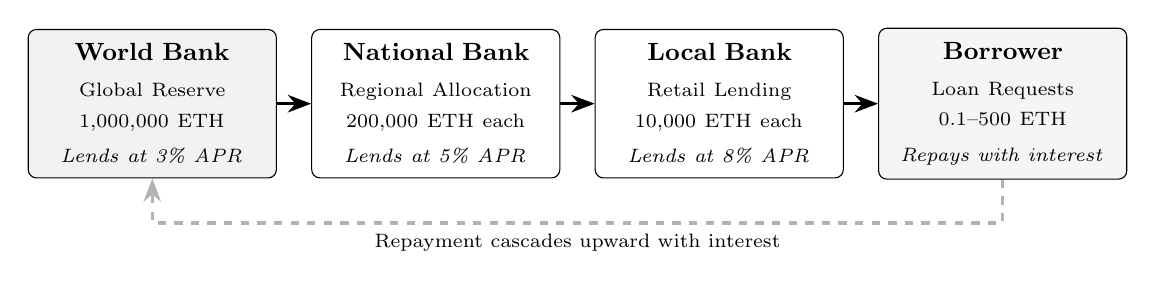
\begin{tikzpicture}[
    tier/.style={
        draw=black,
        fill=white,
        rounded corners=3pt,
        minimum width=3cm,
        minimum height=1.8cm,
        text width=2.8cm,
        align=center,
        font=\small,
        inner sep=5pt,
    },
    tierarrow/.style={
        ->,
        >={Stealth},
        line width=1.2pt,
        color=black,
    },
]
\node[tier,fill=gray!10] (wb) at (0,0) {%
    \textbf{World Bank}\\[2pt]
    {\scriptsize Global Reserve}\\
    {\scriptsize 1,000,000 ETH}\\[2pt]
    {\scriptsize\textit{Lends at 3\% APR}}};

\node[tier] (nb) at (3.6,0) {%
    \textbf{National Bank}\\[2pt]
    {\scriptsize Regional Allocation}\\
    {\scriptsize 200,000 ETH each}\\[2pt]
    {\scriptsize\textit{Lends at 5\% APR}}};

\node[tier] (lb) at (7.2,0) {%
    \textbf{Local Bank}\\[2pt]
    {\scriptsize Retail Lending}\\
    {\scriptsize 10,000 ETH each}\\[2pt]
    {\scriptsize\textit{Lends at 8\% APR}}};

\node[tier,fill=gray!8] (br) at (10.8,0) {%
    \textbf{Borrower}\\[2pt]
    {\scriptsize Loan Requests}\\
    {\scriptsize 0.1--500 ETH}\\[2pt]
    {\scriptsize\textit{Repays with interest}}};

\draw[tierarrow] (wb) -- (nb);
\draw[tierarrow] (nb) -- (lb);
\draw[tierarrow] (lb) -- (br);

\draw[tierarrow,dashed,color=gray!60] (br.south) -- ++(0,-0.55) -| node[below,pos=0.25,font=\scriptsize,color=black] {Repayment cascades upward with interest} (wb.south);
\end{tikzpicture}
\caption{Four-tier hierarchical capital flow with cascading repayment.}
\label{fig:four-tier}
\end{figure}


\section{Auxiliary Dual-Currency Facility}

The cryptocurrency exchange feature of Crypto World Bank is built upon the cryptocurrency exchange facility that is an auxiliary facility incorporated into the current banking infrastructures all over the world. Instead of being a separate exchange, the platform is a service that is provided by all participating banks as an additional service to the existing product portfolio.

\begin{itemize}[noitemsep]
\item \textbf{Integration model:} The dual-currency facility is offered by all participating banks as an add-on service to their existing product portfolio. No additional banking license or separate entity is needed.
\item \textbf{Eligibility determination:} Eligibility of the dual-currency service is based on the bank officers managing the lending operations, on the basis of existing KYC/AML compliance, account status, and lending relationship history.
\item \textbf{No defaulting of conditions:} The project does not override, modify, or default any existing banking conditions, regulatory requirements, or contractual obligations.
\item \textbf{Scope:} The facility enables fiat-to-crypto and crypto-to-fiat conversions, cryptocurrency-denominated lending and repayment, and transparent on-chain transaction records---all within the governance structure of the participating bank.
\end{itemize}

\section{Banking Product Suite}
\label{sec:banking-products}

This section describes the banking products that the platform is designed to support across tiers. While the current prototype implementation focuses primarily on hierarchical lending, the complete system design includes deposit products, transactional accounts, solidarity lending, and multi-currency operations.

\subsection{Savings Products}

The platform offers savings products at the Local Bank tier and, by extension, at higher tiers for institutional participants. Standard savings accounts provide liquid deposits with variable yield tied to platform utilization, allowing deposit pricing to respond to market conditions rather than discretionary rate-setting. Fixed-term deposits lock capital for defined periods (e.g., 30/90/180/365 days) in exchange for a higher agreed yield written into the contract at deposit time. Early withdrawal can be permitted with an automatically enforced penalty (forfeiture of a portion of accrued interest), which is transparent and deterministic.

The yield on standard savings accounts is algorithmically determined by platform utilization: when loan demand is high and available liquidity is low, savings yields rise to attract deposits; when liquidity is abundant, yields fall. This creates a self-regulating capital cycle where savings and lending are linked through a single on-chain formula rather than through discretionary rate-setting committees.

Fixed-term deposits serve a distinct function in the banking architecture: they provide the Local Bank tier with predictable, duration-matched liabilities that can be deployed into longer-term installment loans without creating dangerous asset-liability mismatches. A depositor who locks funds for 180 days effectively funds the 6-month installment tranche of a retail borrower at that tier, eliminating the duration mismatch that causes bank runs in traditional fractional reserve systems.

The closed-loop argument is central to the platform's economic sustainability: unlike donor-funded microfinance models that depend on external capital injections, a savings-funded lending model recycles depositor capital through the lending pool continuously. Interest earned by the platform on loans is partially redistributed to depositors as yield, partially retained as protocol revenue, and partially allocated to the insurance fund, creating a self-sustaining three-way split that does not require new token issuance or external subsidy.

\subsection{Checking and Transactional Accounts}

In addition to interest-bearing savings products, the platform provides transactional accounts (checking/current-account equivalents) for day-to-day financial activity. Transactional accounts carry no yield but impose no lock-in, allow transfers between registered accounts, and serve as the primary account from which loan installments are debited and income receipts are credited. Transfers between accounts within the platform are settled atomically: a transaction either completes fully or reverts, eliminating intermediate settlement ambiguity.

The atomic settlement property of on-chain transfers eliminates the intermediate state that causes the majority of interbank disputes in traditional banking. In the correspondent banking model, a payment can exist in a ``funds in transit'' state for two to five business days during which the sender has debited but the receiver has not credited, creating reconciliation complexity and dispute resolution costs. On-chain transfers settle in a single transaction: either both the debit and credit execute or neither does, with no intermediate state possible.

For retail users in developing economies, transactional accounts on the platform serve as a substitute for the informal cash-handling systems that currently dominate daily financial activity. Recurring payroll deposits, utility payment debits, and peer transfers can all be scheduled as programmable transactions, reducing the friction of cash management without requiring users to interact directly with smart contracts for every operation.

\subsection{Group / Solidarity Lending}

The platform implements a group lending module inspired by the solidarity group model used in microfinance. A group of three to twenty registered borrowers can form a lending group on-chain. Each member contributes collateral into a shared pool; the loan application is submitted collectively; and all members signal consent before escalation to bank approvers. Repayment is tracked per member, and if a member defaults beyond a grace period, the contract can automatically cover the shortfall from the shared collateral pool under programmable mutual liability rules. Over time, group repayment histories contribute to credit scoring to enable progressive lending (larger loans and improved terms after successful cycles).

The group lending module is directly inspired by the solidarity group model developed by BRAC, the organization whose name this university bears. BRAC's group lending program, operating across Bangladesh and subsequently 11 other countries, demonstrates that social collateral (the mutual accountability of group members) can substitute for physical collateral among populations with no formal credit history. The Crypto World Bank translates this social model into programmable contract logic: the mutual liability that BRAC enforces through field officer visits and weekly group meetings is enforced by the GroupLendingPool contract through automatic collateral claims and on-chain consent recording.

The full group loan lifecycle proceeds as follows. First, formation: three to twenty registered borrowers form a group on-chain, each contributing individual collateral to a shared pool contract. Second, application: the group submits a collective loan application specifying the total amount, per-member share, and repayment schedule. Third, consent: every group member must sign the application transaction before it is escalated to a bank approver, enforcing unanimous consent and preventing coerced participation. Fourth, approval: the bank approver reviews the group's aggregate credit history, income verification documents, and shared collateral ratio before approving disbursement. Fifth, disbursement: funds are distributed to each member's account in their individual share as defined by the formula \(\text{Share}_i = \text{LoanTotal} / N_{\text{members}}\). Sixth, repayment: each member repays their individual installments independently; on-chain tracking records per-member performance transparently to all group members. Seventh, mutual liability enforcement: if a member defaults beyond the grace period, the contract automatically covers the shortfall from the shared collateral pool, protecting the lending bank's position while distributing the cost proportionally across the group. Eighth, credit history improvement: successful group repayment cycles are permanently recorded on-chain and incorporated into each member's credit score, enabling progressive lending with larger amounts and better terms in subsequent cycles.

\subsection{Foreign Exchange and Multi-Currency Operations}

A worldwide banking platform must support participants operating in different currency environments. The platform's FX module is designed to use decentralized price oracle networks to obtain verifiable exchange rates for supported asset pairs. Currency conversion can be offered at transparent oracle-derived rates with a disclosed spread, set by governance, that forms an additional revenue stream. To reduce liability-side volatility for retail borrowers, the platform is designed to support stablecoin-denominated lending (e.g., USDC/USDT) while allowing collateral in volatile cryptoassets (e.g., ETH).

\subsection{Trade Finance Facilitation (Planned)}

Trade finance instruments (letters of credit, guarantees, documentary collections) can be added as planned extensions for import--export participants. In a smart contract design, a buyer's bank locks payment in escrow, and release occurs automatically upon verified presentation of shipping documents via trusted data sources. This extension is out of scope for the current prototype but follows the same principles of programmable settlement and auditable execution.

\subsection{Privacy-Preserving Identity Compliance (Planned)}
\label{sec:zkp-compliance}

The regulatory compliance requirements of a worldwide banking platform extend beyond on-chain audit trails. Formal KYC and AML processes require users to prove legal identity, verify source of funds, and satisfy jurisdiction-specific screening requirements. Storing this personal data on a public blockchain creates a fundamental tension between regulatory compliance and user privacy.

The planned resolution is a zero-knowledge proof based KYC layer in which a licensed identity provider performs the full KYC verification off-chain and issues a verifiable credential to the user. The user then presents a ZKP to the banking contracts that proves they hold a valid credential from an approved provider without revealing any personal information on-chain. The contract validates the proof cryptographically and sets a \texttt{kycVerified} flag on the wallet address, enabling access to regulated operations such as large loans, FX conversions, and cross-border transfers. This approach satisfies regulatory requirements while preserving on-chain privacy and avoiding the liability of storing personal financial data in an immutable public record.


\section{Governance Framework}

\subsection{Network Membership Governance}

\begin{table}[H]
\centering
\TableImageMaxFit{3.8.png}
\TableScreenshotEnd
\end{table}

\vspace{2pt}
\noindent\textit{\small This governance table defines membership and onboarding rules that control who can join the banking network and under which role. The structure is intended to preserve institutional accountability by separating responsibilities across tiers rather than relying on undifferentiated token-holder governance alone.}

\subsection{Business Network Governance}

\begin{table}[H]
\centering
\TableImageMaxFit{3.9.png}
\TableScreenshotEnd
\end{table}

\vspace{2pt}
\noindent\textit{\small This business governance table outlines operational controls such as approvals, limits, and escalation paths for higher-risk actions. The goal is to combine programmable enforcement with human oversight, matching real banking governance while retaining on-chain audit trails.}

\subsection{Technology Infrastructure Governance}

\begin{table}[H]
\centering
\TableImageMaxFit{3.10.png}
\TableScreenshotEnd
\end{table}

\vspace{2pt}
\noindent\textit{\small This technology governance table specifies how protocol parameters and infrastructure changes are managed, including security controls and upgrade considerations. It supports the thesis emphasis on safe staged rollout and maintainability under evolving regulatory and security requirements.}

\subsection{Regulatory Compliance Considerations}

As the platform is active in the regulated banking sector:
\begin{itemize}[noitemsep]
\item Our prototype stage would be solely on the \textbf{public testnets} without attached real monetary value.
\item The architecture would facilitate \textbf{audit logs generation} to be reviewed by regulatory regimes on the sandbox programs.
\item Future production deployment would engage \textbf{regulatory sandbox programs} in target jurisdictions.
\end{itemize}

Although the current prototype does not process KYC/AML data, a complete worldwide banking architecture must account for compliance at the design level. Privacy-preserving KYC design is described in detail in Section~\ref{sec:zkp-compliance}.

\subsection{Asset Tokenization}

\begin{itemize}[noitemsep]
\item \textbf{Current implementation:} The native blockchain currency (ETH/MATIC) is used as the reserve and loan currency.
\item \textbf{Planned extension:} Support for ERC-20 stablecoins (USDC, USDT) for lending operations in USD; tokenized collateral instruments for lending situations where there isn't enough collateral.
\end{itemize}

\section{Threat Model and Security Controls}

Security threats in smart-contract banking systems are not limited to isolated code defects; they include economic attacks, oracle manipulation, and governance failure modes. Table~\ref{tab:threat-model} consolidates the primary threat categories considered in the system design and the corresponding controls.

\begin{table}[H]
\centering
\caption{Threat model and security controls mapping}
\label{tab:threat-model}
\begin{tabular}{p{3.2cm}p{6.2cm}p{6.2cm}}
\hline
\textbf{Threat Category} & \textbf{Attack Vector} & \textbf{Implemented / Planned Mitigation} \\
\hline
Reentrancy and state manipulation & External contract calls exploit inconsistent intermediate state during execution (e.g., withdraw patterns) & Use of OpenZeppelin primitives (e.g., \texttt{ReentrancyGuard}); checks-effects-interactions discipline; unit tests covering critical flows \\
\hline
Arithmetic errors & Integer overflow/underflow and unsafe math in financial logic & Solidity~0.8.x built-in overflow protection; explicit bounds checks for rates/limits \\
\hline
Oracle manipulation (planned modules) & Price feed manipulation affecting collateral valuation or FX conversion & Use decentralized oracle networks; medianization and heartbeat checks; conservative risk parameters and circuit breakers for stale / anomalous prices \\
\hline
Sybil abuse (retail / group lending) & Attackers create many wallets to bypass limits or create fraudulent groups & On-chain role binding; rate limits at Local Bank tier; planned compliance gating for higher-risk operations (Section~\ref{sec:zkp-compliance}) \\
\hline
Governance capture & Privileged roles abused to register malicious banks or approve unsafe parameters & Tiered role separation (World Bank / National / Local); immutable audit trails; staged rollout and emergency pause mechanisms under governance \\
\hline
Flash-loan driven economic attacks & Atomic borrowing used to manipulate on-chain state / pricing assumptions & Conservative design for price-dependent logic; oracle protections; monitoring and pause-on-anomaly procedures (planned) \\
\hline
\end{tabular}
\end{table}


%% %%%%%%%%%%%%%%%%%%%%%%%%%%%%%%%%%%%%%%%%%%%%%%%%%%%%%%%%%%%%
%% CHAPTER 4: METHODOLOGY
%% %%%%%%%%%%%%%%%%%%%%%%%%%%%%%%%%%%%%%%%%%%%%%%%%%%%%%%%%%%%%
\chapter{Methodology}

This project and its planning have been structured in accordance with the \href{https://bcolbd.org/uploads/guideline/BLOCKCHAIN\%20OLYMPIAD\%20BANGLADESH\%20AI\%20Guideline.pdf}{Blockchain Olympiad Bangladesh AI guidelines}~[16] and the final-year project evaluation rubrics.

\section{Development Methodology}

We adopted a \textbf{lightweight Agile/Scrum} methodology tailored for an academic prototype with a fixed two-month development window. The iterative approach enables incremental delivery of demonstrable features while accommodating evolving requirements inherent in research-oriented development. Figure~\ref{fig:agile-process} illustrates our Agile process.

\begin{figure}[H]
\centering
\FigureImageMaxFit{Agile Process Diagram.png}
\caption{Agile/Scrum process diagram showing sprint cycles, backlog refinement, and iterative delivery within the 8-week development window.}
\label{fig:agile-process}
\end{figure}

The following points summarize how Agile will be applied:
\begin{itemize}[noitemsep]
\item \textbf{Sprint Duration:} A period of 2 to 3 weeks is allocated for every sprint (3 sprints total).
\item \textbf{Team Size:} A group of two developers will be assigned (thesis project). The work will be focused on the thesis project.
\item \textbf{Weekly Sync:} A weekly gathering will occur to assess progress. Issues will be identified during these meetings. Plans will also be developed in these sessions alongside progress checks.
\item \textbf{Sprint Planning:} Planning for the sprint will take place for one hour at the beginning of every sprint.
\item \textbf{Sprint Review and Retrospective:} Reviewing work occurs at every sprint's conclusion. A discussion on lessons learned will be conducted for 30 minutes.
\end{itemize}

\section{Planned AI/ML Support}

The AI/ML implementation in this prototype phase is scoped to three auditable, lightweight components that provide meaningful decision support without requiring large labeled training datasets.

\begin{itemize}[noitemsep]
\item \textbf{Fraud detection:} Random Forest classifiers assess transaction-level fraud risk based on behavioral and contextual features.
\item \textbf{Anomaly detection:} Isolation Forest detects unusual wallet behavior without requiring labeled fraud samples, making it suitable for data-scarce DeFi environments.
\item \textbf{Explainability:} SHAP generates per-prediction feature attributions that make lending risk assessments interpretable to approvers and regulators.
\end{itemize}

The focus of this prototype phase is establishing the blockchain lending architecture; full ML pipeline development including dataset collection, model training at scale, and production integration is planned for the final thesis phase.

\paragraph{Limitations (prototype and research context).}
The AI/ML components are subject to known limitations in DeFi-like environments. Fraud events are typically rare (class imbalance), and attacker behavior changes over time (concept drift), meaning models trained on historical patterns may degrade without ongoing retraining and monitoring. New wallets also present a cold-start problem with limited behavioral history, and sophisticated adversaries may attempt to structure transactions to evade detection. These limitations motivate conservative use of AI/ML as decision support rather than an automated approval authority in the prototype phase.

\section{Evaluation Methodology}

This section summarizes how each research question will be evaluated in the prototype phase.
\begin{itemize}[noitemsep]
\item \textbf{RQ1 (architecture fidelity):} feature comparison and workflow mapping against flat DeFi protocols (e.g., Aave, Compound, MakerDAO), focusing on institutional hierarchy, role separation, and directional capital flow.
\item \textbf{RQ2 (settlement and transparency):} measurement of transaction latency and approximate per-transaction cost on testnets / Layer~2, plus demonstration of on-chain verifiability of reserves and critical state transitions.
\item \textbf{RQ3 (analytics support):} model evaluation using standard metrics (precision, recall, F1) on available datasets and controlled synthetic cases, alongside qualitative assessment of SHAP explanations.
\item \textbf{RQ4 (technical viability):} end-to-end deployment verification on public testnets with integration tests covering wallet connection, loan request, approval, repayment, and role-based access control.
\item \textbf{RQ5 (banking extensions):} design-level validation via specification completeness and interface contracts for deposit products and group lending, plus prototype demonstrations of selected mechanisms where implemented.
\end{itemize}

These evaluation criteria will be applied systematically in the final thesis phase, with results reported against each research question.

\begin{figure}[H]
\centering
\FigureImageMaxFit{4.2 agile window.png}
\caption{Agile development lifecycle --- 2-month window with three sprints.}
\end{figure}

\begin{figure}[H]
\centering
\FigureImageMaxFit{Methodology.png}
\caption{Technical development methodology: blockchain (Solidity), frontend (React, Wagmi, WalletConnect), backend (Express.js REST API, PostgreSQL), and AI/ML (Python, FastAPI, scikit-learn, Random Forest, SHAP) components across the three sprints.}
\label{fig:methodology-technical}
\end{figure}


\section{Sprint Plan and Deliverables}

\subsection{Sprint 1: Foundation and Core Banking (Weeks 1--3)}

\textbf{Sprint Goal:} Establish core blockchain infrastructure and hierarchical banking structure.

\begin{table}[H]
\centering
\TableImageMaxFit{4.1.png}
\TableScreenshotEnd
\end{table}

\vspace{2pt}
\noindent\textit{\small This sprint planning table breaks Sprint~1 into concrete deliverables that establish the foundation: contract deployment, wallet integration, and the initial data model. The plan is structured to deliver a demonstrable vertical slice early, reducing integration risk for later features.}

\begin{table}[H]
\centering
\TableImageMaxFit{4.2.png}
\TableScreenshotEnd
\end{table}

\vspace{2pt}
\noindent\textit{\small This Sprint~1 continuation clarifies additional tasks and story point allocation for core banking scaffolding. The story point distribution reflects the early emphasis on infrastructure and correctness over feature breadth.}

\textbf{Sprint 1 Total:} 42 story points. Deliverables: smart contracts deployed on testnet, basic frontend with wallet connection, database schema implemented, role-based access control, dashboard UI.


\subsection{Sprint 2: Lending Features and Communication (Weeks 4--6)}

\textbf{Sprint Goal:} Implement complete lending workflow and communication features.

\begin{table}[H]
\centering
\TableImageMaxFit{4.3.png}
\TableScreenshotEnd
\end{table}

\vspace{2pt}
\noindent\textit{\small This Sprint~2 table focuses on completing the lending lifecycle and communication workflows, which are the main user-facing banking operations. The decomposition reflects dependency ordering: workflow correctness precedes advanced analytics integration.}


\subsection{Sprint 3: AI/ML Security and Finalization (Weeks 7--8)}

\textbf{Sprint Goal:} Integrate AI/ML analytics, complete testing, and prepare documentation.

\begin{table}[H]
\centering
\TableImageMaxFit{4.4.png}
\TableScreenshotEnd
\end{table}

\vspace{2pt}
\noindent\textit{\small This Sprint~3 table allocates effort to AI/ML monitoring, testing, and documentation finalization. The intent is to defer analytics complexity until core lending flows are stable, ensuring explainability and auditability can be evaluated against realistic workflows.}

\vspace{4pt}
\noindent\textbf{Additional Sprint~3 module scope (planned):}
\begin{itemize}[noitemsep]
\item \textbf{Group lending module:} architectural design, smart contract interface specification, and partial implementation of group formation and consent recording logic.
\item \textbf{Savings account module:} SavingsVault contract design, interest accrual formula implementation, and interface specification for fixed-term deposits.
\item \textbf{FX module:} oracle integration design and interface specification for dual-currency conversion.
\end{itemize}

Figure~\ref{fig:sprint-submission} shows the sprint submission workflow.

\begin{figure}[H]
\centering
\FigureImageMaxFit{Sprint submission Diagram.png}
\caption{Sprint submission diagram showing the workflow from backlog refinement through development, testing, review, and delivery for each sprint cycle.}
\label{fig:sprint-submission}
\end{figure}


\section{SDLC Stage Mapping}

We map our Agile sprints to the seven stages of the Software Development Life Cycle (SDLC). Figure~\ref{fig:sdlc-mapping} illustrates this mapping.

\begin{table}[H]
\centering
\TableImageMaxFit{4.5.png}
\TableScreenshotEnd
\end{table}

\vspace{2pt}
\noindent\textit{\small This SDLC mapping table aligns the three-sprint Agile plan with standard SDLC stages to ensure research deliverables remain complete (requirements, design, implementation, testing, and evaluation). The mapping makes the development process auditable and easier to justify in an academic setting.}

\begin{figure}[H]
\centering
\FigureImageMaxFit{SDLC stage mapping.png}
\caption{SDLC stage mapping diagram showing alignment between the seven SDLC stages and our three-sprint Agile methodology.}
\label{fig:sdlc-mapping}
\end{figure}


\section{Design Decisions and Alternatives}

For each major design decision, we evaluated alternatives and justified selections based on technical criteria, ecosystem maturity, and project constraints. Figure~\ref{fig:design-decisions} visualizes these comparisons.

\begin{table}[H]
\centering
\TableImageMaxFit{4.6.png}
\TableScreenshotEnd
\end{table}

\vspace{2pt}
\noindent\textit{\small This design decisions table records evaluated alternatives (chains, stacks, libraries) and the criteria used to select the final approach. Documenting these trade-offs strengthens the methodological rigor and clarifies why the selected stack best matches the project's constraints.}

\begin{figure}[H]
\centering
\FigureImageMaxFit{Design Decisions and Alternatives Considered.png}
\caption{Design decisions and alternatives visualization across all major technology choices.}
\label{fig:design-decisions}
\end{figure}

\subsection{Justification of Selected Technologies}

\textbf{1st Choice Justifications:}

\begin{itemize}[noitemsep]
\item \textbf{Agile/Scrum} was necessary due to the project's evolving nature. Frequent updates to smart contract designs, user interface steps and AI/ML connections were required. Adopting Agile allows for plan alterations during brief work cycles effectively avoiding time and resource loss. Significance arises as new concepts emerge during the prototype development process.

\item \textbf{DApp + Off-chain AI} architecture allows intensive machine learning operations to occur outside the blockchain. Machine learning tasks are often run on the blockchain at a considerable expense occasionally exceeding \$100 for a single operation. Off-chain processing enables the use of rapid GPUs along with widely-used Python machine learning resources. Final lending choices are managed exclusively by smart contracts on-chain ensuring that trust is maintained in critical areas.

\item \textbf{React + TypeScript} is beneficial as many Web3 libraries such as Wagmi, RainbowKit, Viem, and ethers.js are supported seamlessly. A vast community of developers exceeding 10~million exists for React making it simpler to access assistance and solutions.

\item \textbf{EVM (Solidity)} is regarded as the most thoroughly examined smart contract system. Over \$100~billion is secured across various blockchains by it. Building and testing the project without incurring costs is possible with free test networks such as Sepolia and Amoy. Security tools provided by OpenZeppelin have been thoroughly tested to ensure the protection of contracts.

\item \textbf{MUI (Material Design~3)} provides ready-made components for typical banking interface designs. The package contains various items such as data tables, form checks and layouts for dashboards. Utilizing MUI results in a time saving of around 40\% compared to starting from scratch.

\item \textbf{Random Forest} performs effectively alongside SHAP's TreeExplainer which swiftly computes precise Shapley values for tree models. Precise calculations are essential for adhering to regulations concerning decision-making transparency. Avoiding approximate methods ensures explanations remain stable which prevents issues during audits.

\item \textbf{Isolation Forest} does not require labeled data for training. Labeled fraud samples are few making it suitable for DeFi lending. Anomalies in transactions are scored swiftly as it operates with a time complexity of $O(n \log n)$.

\item \textbf{SHAP} provides feature importance through solid mathematical foundations from game theory (Shapley values). Characteristics such as accuracy, management of absent data and consistency are not assured by tools like LIME. These properties assist in fulfilling emerging regulations for explainable decisions within financial services.

\item \textbf{PostgreSQL} effectively manages complex time-based queries. Borrowing limits can be checked over periods such as 6 months or 1 year. ACID compliance is fully supported to ensure financial data remains secure. It supports JSON which facilitates easy adjustments to the database structure during the prototyping phase.

\item \textbf{Vercel + Render} facilitates deploying the demo globally at no charge. A live prototype can be accessed without the necessity of a setup on personal computers. Supervisors, examiners and other individuals are not required to deal with installation issues.
\end{itemize}

\textbf{2nd Choice Justifications (Why Retained as Alternatives):}

\begin{itemize}[noitemsep]
\item \textbf{Incremental (Waterfall) methodology} produces more predictable and clearly phased deliverables. However, it offers limited capacity to adapt to the evolving requirements typical of research-oriented prototype development, and is most effective in stable production environments where scope is fixed from the outset.

\item \textbf{Hybrid with Oracle architecture} (e.g., Chainlink) would enable on-chain ML prediction triggers via oracle data feeds, increasing the verifiability of AI-driven decisions. The trade-off is meaningful latency (30--60 seconds per update) and additional cost (\$0.10--1.00 per oracle call), along with a dependency on third-party oracle availability that introduces an external failure point not present in the selected off-chain approach.

\item \textbf{Vue + TypeScript} is approachable for developers new to JavaScript frameworks. Its Web3 tooling ecosystem (e.g., vue-dapp) is less mature than React's, with sparser wallet integration library support and slower update cadence for critical Web3 dependencies.

\item \textbf{Solana (Rust)} offers substantially higher raw throughput (up to 65,000 TPS) than EVM-compatible chains. However, Solana's developer tooling and security library ecosystem are less established, the Rust learning curve is significant within an 8-week development window, and the DeFi security audit tooling available for Solidity (Slither, Mythril, OpenZeppelin) has no direct equivalent on Solana.

\item \textbf{Tailwind CSS} offers greater design flexibility through utility-first composition. Achieving consistent, professional banking-style UI patterns requires substantially more custom work than using MUI's pre-built component library, which imposes a time cost that is unacceptable within the sprint timeline.

\item \textbf{XGBoost} frequently outperforms Random Forest on structured tabular datasets. However, its SHAP integration uses approximate rather than exact tree computation, meaning explanations cannot be guaranteed to be consistent across repeated evaluations---a property required for regulatory auditability of credit decisions.

\item \textbf{Autoencoder} models can capture complex non-linear anomaly patterns. In practice, they require substantial labeled or unlabeled training data and careful hyperparameter tuning to converge reliably. Isolation Forest is parameter-light and performs competitively on small and imbalanced datasets, making it better suited to the data-scarce DeFi lending context of this prototype.

\item \textbf{LIME} produces faster local explanations. As demonstrated by Adom et al.~[4], LIME explanations are unstable: repeated evaluation of the same input can yield different feature importance rankings, undermining the consistency guarantees that regulators require for automated lending decisions.

\item \textbf{SQLite} eliminates database infrastructure overhead and is straightforward to configure. It does not support concurrent writes, which limits multi-user prototype testing, and lacks the window function and CTE support needed for rolling 6-month and 1-year borrowing limit calculations.

\item \textbf{Localhost-only deployment} removes hosting dependencies and infrastructure cost. It prevents remote sharing for supervisor review, collaborative testing across team members, and examiner access to a live demo---all of which are necessary for academic evaluation and iteration.
\end{itemize}


\section{Design Patterns}

Our system uses three design patterns:

\begin{itemize}[noitemsep]
\item \textbf{Singleton:} A singleton means that each primary contract is established a single time. Only one version is utilized by all ensuring a unified source of truth. Not everyone can create multiple versions of the contract.

\item \textbf{Observer:} Contracts generate alerts whenever actions occur such as loan requests. These alerts are processed by a service that updates the database. Notifications are not ignored; they receive attention.

\item \textbf{Adapter:} An Adapter is utilized by the wallet component to function with various wallet types (like MetaMask). Different wallets that adhere to the EIP-1193 standards can be easily integrated.

\item \textbf{Factory Pattern:} Each Local Bank creates individual loan and savings contract instances using a factory contract, ensuring all deployed instances follow the same security-audited interface and access control checks. The factory pattern prevents unauthorized contract deployment that could bypass the hierarchical governance structure.

\item \textbf{Proxy/Upgradeable Pattern:} Banking contracts must be upgradeable without losing stored state such as balances, credit scores, and loan histories. OpenZeppelin's transparent proxy pattern separates the contract's logic from its storage, allowing governance-approved upgrades to the logic layer while preserving all stored financial data. This pattern is essential for a long-lived banking system that must adapt to evolving regulatory requirements and security patches.
\end{itemize}


\section{Software Testing Strategy}

The testing strategy covers four layers of the system, each with defined acceptance criteria.

\begin{itemize}[noitemsep]
\item \textbf{Smart contract unit tests:} Numerous tests for smart contracts exist in our Hardhat environment. Over 12 tests are conducted to verify actions related to managing reserves, sign-ups, loans and access permissions. No scenarios such as depositing zero or executing disallowed actions are missed in these assessments. \textbf{Acceptance criterion:} all Hardhat unit tests pass with zero failures before any sprint delivery.
\item \textbf{Integration testing:} Whole process checks are conducted for integration tests. Wallet connection, loan request, approval and repayment processes are evaluated on the network. No critical steps are excluded from the process. \textbf{Acceptance criterion:} end-to-end workflow completes successfully on testnet for representative scenarios (approval, rejection, repayment loop).
\item \textbf{AI/ML module verification:} Ensuring functionality is vital for our fraud and unusual activity detectors. Results are generated by the integration of the detectors with the overall system. \textbf{Acceptance criterion:} model inference endpoints return valid scores and explanations for test inputs without runtime errors.
\item \textbf{Frontend testing:} Website appearance is evaluated on Chrome, Firefox and mobile devices. Tests are conducted to ensure that functionality is maintained across various platforms. \textbf{Acceptance criterion:} core flows render and remain usable across desktop and mobile breakpoints without blocking UI defects.
\end{itemize}


%% %%%%%%%%%%%%%%%%%%%%%%%%%%%%%%%%%%%%%%%%%%%%%%%%%%%%%%%%%%%%
%% CHAPTER 5: MARKET ANALYSIS AND FEASIBILITY
%% %%%%%%%%%%%%%%%%%%%%%%%%%%%%%%%%%%%%%%%%%%%%%%%%%%%%%%%%%%%%
\chapter{Market Analysis and Feasibility}

\section{Market Sizing}

\begin{table}[H]
\centering
\TableImageMaxFit{5.1.png}
\TableScreenshotEnd
\end{table}

\vspace{2pt}
\noindent\textit{\small This table quantifies the demand-side context (DeFi lending, remittances, MSME credit gap) used to ground the feasibility argument in measurable market data. It shows the platform targets both a high-volume settlement problem and a persistent inclusion/credit-access gap.}

\vspace{4pt}
\noindent\textit{\small\textbf{Sources:} (a)~TAM: DefiLlama~[13] reports DeFi lending TVL exceeding \$55~billion; World Bank Migration and Development Brief~[26] values global remittances at \$860~billion annually; IFC~[20] estimates the MSME financing gap at \$4.5~trillion; (b)~SAM and SOM: project-derived estimates based on industry segmentation of institutional lending and regulatory sandbox addressable market~[18].}

No hierarchically structured lending system currently exists in DeFi; existing protocols rely on undifferentiated shared pools. Cross-border payment networks such as Ripple (\$847M daily)~[25] and JPMorgan Kinexys (\$3--7B daily)~[40] handle settlement volume but offer no lending, deposit, or tiered governance functions. Institutional interest in blockchain-based finance is clearly established, yet no single platform combines DeFi-style accessibility with the structured capital hierarchy of traditional development banking. The Crypto World Bank is designed to occupy this gap.

\section{Target Customer Segment}

The Crypto World Bank targets the \textbf{retail customer segment}---individual borrowers and small businesses seeking transparent, accessible crypto-based lending services.

\begin{table}[H]
\centering
\TableImageMaxFit{5.2.png}
\TableScreenshotEnd
\end{table}

\vspace{2pt}
\noindent\textit{\small This target-customer table articulates the retail borrower profile and constraints that drive product requirements (low fees, simple onboarding, transparent terms). It supports the decision to prioritize usability and cost efficiency over complex institutional-only features in the prototype phase.}

\section{Partner Ecosystem}

\begin{table}[H]
\centering
\TableImageMaxFit{5.3.png}
\TableScreenshotEnd
\end{table}

\vspace{2pt}
\noindent\textit{\small This partner ecosystem table highlights external dependencies (identity/verification flows, infrastructure, and settlement rails) needed for a real deployment. Identifying these actors early reduces hidden-scope risk and clarifies what remains outside the smart contract boundary.}


\section{Competitive Landscape}

The Crypto World Bank operates at the intersection of four distinct competitor categories. Table~\ref{tab:competitor-detailed} provides a detailed comparison of representative projects in each category, with current metrics as of March~2026.

\begin{table}[H]
\centering
\TableImageMaxFit{5.4.1.png}
\TableScreenshotEnd[tab:competitor-detailed]
\end{table}

\vspace{2pt}
\noindent\textit{\small This competitive landscape table compares representative projects across DeFi lending, payment rails, inclusion wallets, and institutional blockchain systems. The comparison highlights the whitespace: no competitor combines hierarchical multi-tier lending with governance-aware controls and AI-assisted monitoring in one architecture.}

\begin{table}[H]
\centering
\TableImageMaxFit{5.4.2.png}
\TableScreenshotEnd
\end{table}

\vspace{2pt}
\noindent\textit{\small This continuation expands the competitor comparison to additional platforms and feature dimensions. It reinforces the thesis positioning by showing that existing systems typically specialize in one function (lending or payments) rather than a complete banking suite.}

\begin{table}[H]
\centering
\TableImageMaxFit{5.4.3.png}
\TableScreenshotEnd
\end{table}

\vspace{2pt}
\noindent\textit{\small This final competitor table block concludes the comparative analysis and clarifies why multi-tier capital flow is a differentiating architectural feature. The results inform the go-to-market focus on transparency, governance structure, and retail accessibility.}

Upon reviewing various projects a common feature was identified: a lending mechanism does not exist that operates with tiers, is distributed and facilitates transactions across different levels and within identical levels. Such innovation distinguishes the Crypto World Bank. The key differentiating features of the Crypto World Bank are as follows:

\begin{itemize}[noitemsep]
\item Existing DeFi lending protocols provide capital access but lack institutional hierarchy, tiered governance, and structured capital flow.
\item Credit platforms such as Maple and Goldfinch engage in lending based on credit. Credit-based lending is often focused on businesses and exists at just one tier. These platforms do not cater to personal loans.
\item Ripple processes cross-border payments but does not offer lending, deposit, or hierarchical capital allocation services.
\item Celo provides assistance to individuals in emerging economies. Payment and savings functions are offered yet lending services remain absent.
\item \textbf{Central Bank Digital Currencies (CBDCs):} The development of CBDCs aims to improve payment systems~[5]. Concerns about privacy and control are raised as lending features are excluded. A lending layer does not exist on a CBDC. Users benefit from our platform which safeguards their interests while providing a level-based system similar to that utilized by CBDCs~[5].
\end{itemize}

\section{Risk Taxonomy}

\begin{table}[H]
\centering
\TableImageMaxFit{5.5.png}
\TableScreenshotEnd
\end{table}

\vspace{2pt}
\noindent\textit{\small This risk taxonomy table categorizes technical, financial, regulatory, and operational risks relevant to an on-chain banking platform. The taxonomy is used to justify design mitigations such as reserve enforcement, role-based approvals, and staged deployment through testnets and sandbox programs.}


\section{Technical Feasibility}

\begin{table}[H]
\centering
\TableImageMaxFit{5.6.png}
\TableScreenshotEnd
\end{table}

\vspace{2pt}
\noindent\textit{\small This technical feasibility table summarizes the readiness of core infrastructure (EVM tooling, Layer~2 scalability, and security libraries) required by the prototype. It supports the claim that the project leverages mature ecosystems rather than experimental primitives, reducing implementation risk.}

The technical feasibility of the platform rests on five pillars: the maturity of the underlying blockchain infrastructure, the availability of development tooling and security primitives, the demonstrated scalability of Layer~2 networks for financial applications, the precedent of comparable institutional blockchain deployments, and the platform's modular architecture which allows incremental delivery without requiring the full system to be operational before any component can be tested.

Ethereum---the EVM standard on which the platform is built---has operated continuously since 2015, while Polygon PoS has processed billions of transactions with low fees and rapid finality, making it suitable for high-frequency retail operations. The contract layer uses established security primitives (e.g., OpenZeppelin libraries and widely reviewed patterns), and the off-chain services use standard, production-grade web tooling for API and ML inference. Because the architecture is modular, components such as savings, FX, group lending, and insurance can be developed and validated independently and integrated through governance-approved rollouts.

\section{Economic Feasibility}

\begin{table}[H]
\centering
\TableImageMaxFit{5.7.png}
\TableScreenshotEnd
\end{table}

\vspace{2pt}
\noindent\textit{\small This economic feasibility table captures cost drivers (gas, infrastructure, and defaults) and compares them against revenue potential from interest spreads and fees. The key conclusion is that low-fee Layer~2 deployment makes small-loan banking workflows economically viable, unlike high-fee base layers.}

The economic feasibility of the platform is evaluated across four dimensions: operational cost sustainability, revenue sufficiency, capital efficiency, and macroeconomic impact. On Polygon PoS, the total on-chain gas cost for a full retail loan lifecycle is measured in cents, while interest spread revenue is orders of magnitude larger, yielding a favorable cost-to-revenue profile for small loans that are infeasible on high-fee base layers. Off-chain infrastructure costs (hosting, RPC access, storage, ML inference) are comparable to typical SaaS deployments and scale with usage.

Revenue is diversified across interest spreads, origination fees, and potential FX spread revenue for multi-currency conversions. Capital efficiency is enhanced by the platform's reserve-enforced fractional allocation and by reducing the need for idle pre-funded balances typical of correspondent banking. At scale, remittance cost reduction and improved access to credit in underserved markets produce additional social and economic value beyond platform revenue.

\section{Revenue Projection}

The following projection models annual revenue potential at full deployment scale. Calculations use a reference ETH price of \textbf{\$2,000} (February 2026 market rate) and interest rate parameters defined in Section~\ref{sec:interest-rates}.

\begin{table}[H]
\centering
\TableImageMaxFit{5.8.png}
\TableScreenshotEnd
\end{table}

\vspace{2pt}
\noindent\textit{\small This revenue projection table provides modeled annual income under a reference ETH price and assumed utilization, default rates, and tier spreads. It illustrates how hierarchical spreads across tiers accumulate into platform-level revenue while keeping retail APR within plausible ranges.}

\begin{table}[H]
\centering
\TableImageMaxFit{5.9.png}
\TableScreenshotEnd
\end{table}

\vspace{2pt}
\noindent\textit{\small This continuation details additional projection assumptions and sensitivity inputs (fees, defaults, and infrastructure cost). Explicit assumptions are necessary for reproducibility and for interpreting the projections as scenario-based estimates rather than guarantees.}

\vspace{4pt}
\noindent The projection above models interest spread income only. Additional revenue streams from FX conversion spreads (estimated 0.5 to 1.0\% per conversion), loan origination fees (1 to 2\% of principal at disbursement), insurance fund premiums (0.5\% of loan value annually), and governance operations represent material upside not captured in this base case. Including these streams would increase projected platform revenue by an estimated 25 to 40\% at equivalent lending volume.

\vspace{4pt}
\noindent\textit{\small\textbf{Sources:} ETH price from spot market data (CoinGecko); interest rate tiers aligned with Aave~[15] and Compound~[16] DeFi benchmarks; default rate and origination fee from conservative industry estimates.}

\vspace{6pt}
\noindent\textbf{Cost Model Considerations.}

\begin{itemize}[noitemsep]
\item \textbf{Gas costs:} Gas expenses on Polygon PoS are quite low. A loan's entire process including request, approval, payment and 12 monthly installments results in costs under \$0.15. Interest income amounts to less than 0.01\% of our earnings. For Ethereum, loan costs may range from \$50 to \$750 influenced by network congestion. Processing transactions in batches or utilizing Layer~2 would be essential for the viability of small loans.
\item \textbf{Infrastructure costs:} Backend hosting (API server, database, ML service), frontend delivery (CDN) and RPC nodes (Alchemy, Infura) can incur costs ranging between \$500 and \$2,000 monthly. An increase in expenses will be experienced with a rise in transactions.
\item \textbf{Default losses:} A default rate of 3\% is anticipated. Approximately \$6.7~million annually is projected as the platform sees heavy usage. Anticipated earnings have already incorporated this amount.
\item \textbf{Break-even analysis:} Opportunities for profit on loans as small as 0.01~ETH (\$20) exist on Polygon PoS. Profitability on loans below 5~ETH (\$10,000) is not achievable on Ethereum without Layer~2. Layer~2 is essential for facilitating small loans.
\end{itemize}

\begin{figure}[H]
\centering
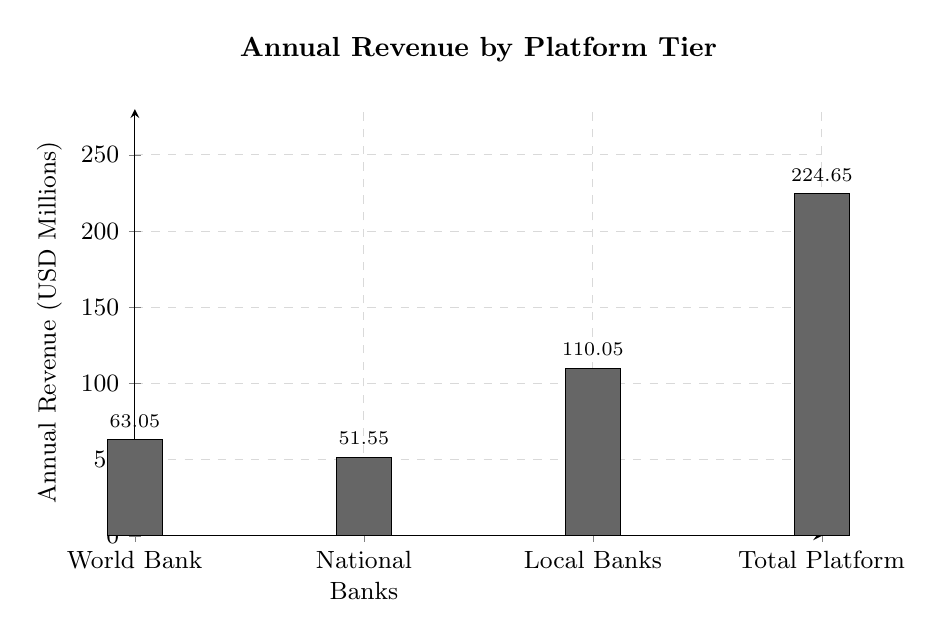
\begin{tikzpicture}
\begin{axis}[
    ybar,
    bar width=20pt,
    width=0.85\textwidth,
    height=7cm,
    clip=false,
    ylabel={Annual Revenue (USD Millions)},
    ylabel style={font=\small},
    symbolic x coords={World Bank,National Banks,Local Banks,Total Platform},
    xtick=data,
    xticklabel style={font=\small,text width=2.2cm,align=center},
    yticklabel style={font=\small},
    ymin=0,
    ymax=280,
    ytick={0,50,100,150,200,250},
    nodes near coords,
    nodes near coords style={font=\scriptsize\bfseries},
    every node near coord/.append style={anchor=south,yshift=1pt},
    enlarge x limits=0.30,
    grid=major,
    grid style={dashed,gray!30},
    axis lines=left,
    title={\textbf{Annual Revenue by Platform Tier}},
    title style={font=\normalsize,at={(0.5,1.05)}},
]
\addplot[fill=black!60,draw=black] coordinates {
    (World Bank,63.05) (National Banks,51.55) (Local Banks,110.05) (Total Platform,224.65)
};
\end{axis}
\end{tikzpicture}
\caption{Annual revenue projection by tier (USD millions, at \$2{,}000/ETH).}
\end{figure}

\subsection{Transaction Economics: Interest Rates}
\label{sec:interest-rates}

\begin{table}[H]
\centering
\TableImageMaxFit{5.10.png}
\TableScreenshotEnd
\end{table}

\vspace{2pt}
\noindent\textit{\small This interest rate table defines the tiered APR parameters used throughout the feasibility and revenue modeling. Presenting the rate structure explicitly makes the spread logic auditable and connects the economic model directly to the proposed governance-controlled parameters.}

\begin{figure}[H]
\centering
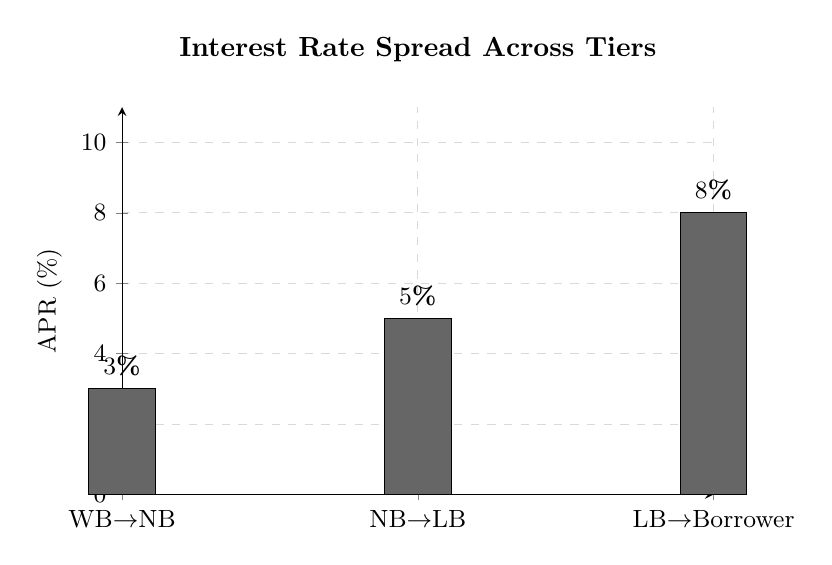
\begin{tikzpicture}
\begin{axis}[
    ybar,
    bar width=24pt,
    width=0.75\textwidth,
    height=6.5cm,
    clip=false,
    ylabel={APR (\%)},
    ylabel style={font=\small},
    symbolic x coords={WB$\to$NB,NB$\to$LB,LB$\to$Borrower},
    xtick=data,
    xticklabel style={font=\small},
    yticklabel style={font=\small},
    ymin=0,
    ymax=11,
    ytick={0,2,4,6,8,10},
    nodes near coords={\pgfmathprintnumber\pgfplotspointmeta\%},
    nodes near coords style={font=\small\bfseries},
    every node near coord/.append style={anchor=south,yshift=1pt},
    enlarge x limits=0.50,
    grid=major,
    grid style={dashed,gray!30},
    axis lines=left,
    title={\textbf{Interest Rate Spread Across Tiers}},
    title style={font=\normalsize,at={(0.5,1.05)}},
]
\addplot[fill=black!60,draw=black] coordinates {
    (WB$\to$NB,3) (NB$\to$LB,5) (LB$\to$Borrower,8)
};
\end{axis}
\end{tikzpicture}
\caption{Hierarchical interest rate spread (APR) across the four-tier lending structure.}
\end{figure}

\subsection{Global Economic Impact}

Apart from revenue generated through platforms, various economic advantages are provided by the Crypto World Bank:

\begin{itemize}[noitemsep]
\item \textbf{Capital deployment and fiscal multiplier:} At projected full-deployment lending volume of \$2~billion across nearly 1,000 institutional borrowers, the platform generates a downstream fiscal multiplier of approximately \$2.5 to \$3 per dollar lent~[19], implying \$5 to \$6~billion in annual economic activity. The IFC estimates that every \$1~million lent to small businesses in developing economies creates approximately 16 new jobs~[20], making capital deployment at this scale a meaningful driver of employment and local economic growth.

\item \textbf{Remittance cost reduction:} Global remittances total approximately \$860~billion annually, of which an estimated \$48 to \$56~billion is consumed by transfer fees averaging 6.49\%---more than double the United Nations Sustainable Development Goal target of 3\%~[26]. On-chain settlement on Layer~2 networks reduces transaction costs to well below 1\%, directly compressing this fee burden. Comparable blockchain payment networks demonstrate the feasibility of this target: Stellar processed approximately \$55.6~billion in payments at a fee of roughly \$0.0007 per transaction in 2025~[44], and Celo's MiniPay processes payments for under one cent across more than 60 countries~[42].

\item \textbf{Trapped capital liberation:} The correspondent banking system requires banks to maintain pre-funded nostro and vostro accounts in every currency corridor in which they operate, immobilizing large sums that cannot be deployed for lending or investment~[24]. On-chain atomic settlement eliminates the need for these idle pre-funded balances, freeing capital for productive use across the lending hierarchy.

\item \textbf{Financial inclusion:} The platform is designed for accessibility: sub-cent gas fees on Polygon PoS, a mobile-first interface, and support for micro-loan amounts below one dollar lower the barriers to credit for the estimated 1.4~billion adults globally who remain outside formal financial systems~[14]. The World Economic Forum has identified decentralized finance as a leapfrog technology capable of enabling populations to bypass the infrastructure constraints of traditional banking~[41], a pattern already observed in mobile payments across developing economies.

\item \textbf{Transaction cost reduction:} On Polygon PoS, transaction fees remain below one cent---a reduction of over \textbf{99\%} relative to the average \$42 cost of a correspondent banking transaction~[25]. This cost compression makes financially viable a large class of micro-transactions and small-loan servicing operations that are currently uneconomical through traditional payment rails.

\item \textbf{Transparency as an economic good:} On-chain publication of reserve ratios, interest rates, and transaction records eliminates the informational asymmetry that enables predatory lending practices in opaque banking environments. In conventional banking, borrowers---particularly in developing economies---frequently operate without visibility into the true cost of credit or the basis for lending decisions. The Crypto World Bank's design ensures that all participants access identical, verifiable information, reducing the scope for hidden fees and unfair pricing.
\end{itemize}

\subsection{Value Proposition and Go-to-Market}

\begin{table}[H]
\centering
\TableImageMaxFit{5.11.png}
\TableScreenshotEnd
\end{table}

\vspace{2pt}
\noindent\textit{\small This value proposition table summarizes user-visible benefits (cost, transparency, speed, and inclusion) and maps them to platform features. It supports the go-to-market narrative by linking technical design choices to practical outcomes for retail users and partner institutions.}


\section{Prototype Scope and Limitations}

A straightforward version of the complete system is represented by the current prototype:

\begin{enumerate}[noitemsep]
\item \textbf{Hierarchical lending scope:} Utilization of the Tier~1 World Bank Reserve contract is comprehensive. Deposits are managed, loan requests and approvals are processed alongside the display of reserve statistics. Not all functions of the Tier~2 (National Bank) and Tier~3 (Local Bank) contracts have been implemented. Role management and registration are not the only aspects focused on. Currently the process for fund transfers from the World Bank to National Bank and subsequently to Local Bank is incomplete. Four tiers will be included in the final design.

\item \textbf{Interest accrual and repayment:} Rules for interest rates (3\%/5\%/8\%) are part of the system design. Fees for initiating loans and penalties for delays also exist. Interest calculations, payment schedules or penalties aren't managed automatically by current smart contracts. Future updates will incorporate these functions.

\item \textbf{InterBankLendingPool and multi-directional flows:} Plans for interbank loans at equal tier levels are included in the design (Section~1.7). Smart contracts have yet to be created for those components. Currently the prototype does not prioritize the upward transfer of funds.

\item \textbf{AI/ML integration:} AI tools such as fraud detection (Random Forest) and anomaly detection (Isolation Forest) along with decision explanations (SHAP) are set to be utilized by the system. A service has been established with FastAPI for machine learning. This service does not currently link to the loan approval process in the existing version.

\item \textbf{Backend architecture:} Express.js paired with MongoDB is utilized for rapid API development. The main database is intended to be PostgreSQL. FastAPI is utilized by the machine learning service.

\item \textbf{Banking product suite:} The extended banking product suite described in Section~\ref{sec:banking-products}, including savings accounts, fixed-term deposits, transactional accounts, group lending, FX conversion, and the insurance fund, is specified at the architectural and design level in this report. Smart contract implementation and testing of these modules is planned for the final thesis phase. The current prototype establishes the hierarchical lending foundation upon which these modules will be integrated.
\end{enumerate}

The limitations above are consistent with a pre-thesis prototype; the complete system design is fully specified in this report and will be implemented and validated in the final thesis phase.


%% %%%%%%%%%%%%%%%%%%%%%%%%%%%%%%%%%%%%%%%%%%%%%%%%%%%%%%%%%%%%
%% CHAPTER 6: CONCLUSION
%% %%%%%%%%%%%%%%%%%%%%%%%%%%%%%%%%%%%%%%%%%%%%%%%%%%%%%%%%%%%%
\chapter{Conclusion}

The Crypto World Bank addresses a \textbf{multi-party coordination and trust} problem inherent in hierarchical development finance by exploiting the distinctive properties of blockchain technology: cryptographic integrity, immutability, and programmable auditability. It advances beyond existing DeFi lending protocols---which collectively manage over \$55~billion in TVL~[13] but universally employ flat, single-tier pool architectures---through a four-tier institutional hierarchy with cross-tier, same-tier, and upward lending flows, combined with a governance structure that addresses network membership, business operations, and technology infrastructure.

The analysis of the competitive situation of 20+ existing projects in DeFi lending, institutional credit, banking infrastructure and financial inclusion affirm that no current system is a combination of multi-level lending (hierarchy), interbank lending mechanisms and graded access by borrowers in one decentralized architecture. The growing blockchain implementation in the institutions, as demonstrated by the World Bank FundsChain initiative~[39], the multi-billion-dollar daily volumes of JPMorgan Kinexys~[40] and R3 Corda's \$17~billion in tokenized assets~[37]---validates both the technical feasibility and institutional demand of blockchain-based financial infrastructure. The Crypto World Bank extends this trajectory from settlement and fund tracking into a fully open, hierarchically governed lending system.

The platform occupies the intersection of institutional finance, decentralized lending, and financial inclusion, a combination that remains unaddressed in both the academic literature and the commercial blockchain landscape. With a working prototype, a defined market and partnership plan, and a planned go-to-market plan, the Crypto World Bank represents a structurally distinct and architecturally grounded contribution to the emerging field of blockchain-based development finance.

Viewed as a complete banking function checklist, the current prototype implements hierarchical lending workflow foundations (tiered roles, governance framing, architectural capital flow, and a planned AI/ML monitoring layer) while leaving several bank-grade modules at the design level. Unimplemented modules specified in this report include:
\begin{itemize}[noitemsep]
\item Deposit products (SavingsVault and FixedDeposit)
\item Transactional accounts (CurrentAccount)
\item Group lending (GroupLendingPool)
\item Oracle-priced FX conversion (FXModule)
\item Interbank liquidity pools (InterBankLendingPool, planned)
\item Insurance and depositor protection (InsuranceFund)
\end{itemize}
Future iterations therefore focus on completing end-to-end cross-tier fund transfers and repayment automation, integrating the analytics layer into real approval flows, and expanding the platform into a functionally complete worldwide banking system with compliance-aware architecture.

The future work will be directed towards the following directions:

\begin{enumerate}[noitemsep]
\item \textbf{Complete hierarchical lending implementation:} Complete the end-to-end wiring of cross-tier fund transfers between the World Bank Reserve, National Bank and Local Bank contracts, including automated capital distribution, interest accrual, generation of installments schedules, generation of cascading repayments enforcement as intended in the architecture.
\item \textbf{InterBankLendingPool and multi-directional flows:} Adopt the same-tier interbank lending pool and upward surplus repatriation mechanisms described in Section~1.7, so as to permit a full modeling of real-life banking liquidity flows in the decentralized structure.
\item \textbf{AI/ML pipeline integration:} Integrate the ML inference based on FastAPI service (Random Forest fraud detection, Isolation Forest anomaly detection, SHAP explainability) into the real-life loan approval process, integrating off-chain on-chain lending decisions to risk assessments.
\item \textbf{Mainnet and regulatory sandbox:} Moving off the testnet to the mainnet featuring real asset testing in regulated sandbox settings (e.g. UK FCA Digital Securities Sandbox, MAS FinTech Regulatory Sandbox Singapore, Bangladesh Bank FinTech Regulatory Sandbox).
\item \textbf{Advanced risk monitoring:} Once the core lending workflow is stable and the blockchain architecture fully implemented, extend the ML monitoring layer to include graph neural network transaction analysis for coordinated fraud ring detection, federated learning across National and Local Banks for privacy-preserving cross-institution threat intelligence, and reinforcement learning agents for adaptive interest rate parameter governance.
\item \textbf{Cross-chain interoperability:} Ethereum Layer~2 multi-network lending rollups (Arbitrum, Optimism, Base) and other EVM chains to serve other geographic markets having optimized gas costs and local regulatory compliance.
\item \textbf{Formal security checking:} Formal verification of all smart contract code based on symbolic execution (Mythril), and static analysis (Slither), formal verification of property (Certora), especially multi-tier lending invariants such as cascading reserve ratio maintenance and cross-tier interest rate bound enforcement.
\item \textbf{Stablecoin integration, fiat on/off-ramps:} Support established blockchain coins (USDC, USDT, DAI) and native blockchain coins, with fiat on/off-ramping by collaborating with licensed money transmitters or anchor networks like MoneyGram that Stellar has implemented~[44].
\item \textbf{Economic simulation and stress testing:} Agent-based simulation of the hierarchical lending system under market stress conditions (bank runs, cascading liquidations, correlated collateral devaluation) to prove convergence of interest rates, adequacy in the reserve ratios, and stability in the system.
\item \textbf{Complete banking product suite implementation:} Develop and deploy the SavingsVault, FixedDeposit, GroupLendingPool, FXModule, InsuranceFund, and CurrentAccount contracts, completing the full nine-contract banking architecture described in Chapter~3. Each module will be validated independently on testnet before integration testing with the existing three-contract lending core.
\item \textbf{On-chain credit history portability:} Implement an open credit score standard that allows borrowers' on-chain repayment history to be recognized by any platform that adopts the standard, creating a portable, self-sovereign financial identity that outlasts any single platform and contributes to solving the credit history gap that excludes 1.4~billion unbanked adults from formal financial systems.
\end{enumerate}


%% %%%%%%%%%%%%%%%%%%%%%%%%%%%%%%%%%%%%%%%%%%%%%%%%%%%%%%%%%%%%
%% APPENDICES
%% %%%%%%%%%%%%%%%%%%%%%%%%%%%%%%%%%%%%%%%%%%%%%%%%%%%%%%%%%%%%
\appendix

\chapter{Technology Stack}

\section{In-product assistant: local large language model (LLM) integration (prototype)}

\paragraph{Purpose.}
The web application includes a streaming chat assistant to help users understand platform concepts (e.g., the four-tier capital hierarchy), screen-specific workflows, and navigation. During local development, the assistant is served by a \textbf{local OpenAI-compatible inference server} (LM Studio) running a quantized Gemma-family model, while the public browser traffic is still routed through the project API to keep keys off the client and to centralize request shaping (system prompts, optional authenticated user context, and error handling).

\paragraph{Model and runtime (local development).}
The inference endpoint follows the \textbf{OpenAI Chat Completions} contract (\texttt{/v1/chat/completions}) with \texttt{stream: true}, proxied from the project backend to a local service such as \texttt{http://127.0.0.1:1234}. The served checkpoint is configured as a Gemma-4 E4B variant (e.g., \texttt{google/gemma-4-e4b}) in GGUF form with a practical quantization (e.g., \texttt{Q4\_K\_M}) for a laptop-friendly footprint (on the order of single-digit GBs). The exact quantization label and on-disk name are a deployment artifact; what matters for integration is the \textbf{API model identifier} exposed by the local server and referenced by the backend configuration (environment-driven).

\paragraph{End-to-end behavior.}
The user interface assembles a short transcript (user/assistant messages) and posts it to the backend streaming route. The backend prepends a \textbf{system message} with platform + screen ``feature'' context, optionally enriched by user role when a valid session token is present. The backend then opens a streaming request to the local model server, converts upstream token events into \textbf{server-sent events (SSE)} for the browser, and the UI incrementally appends text. The message renderer uses Markdown (including GitHub-flavored extensions), math (KaTeX) for \texttt{\$\$...\$\$} blocks, and line-break rules appropriate for chat transcripts.

\paragraph{Security and limitations (prototype stance).}
The assistant is a \textbf{read-only product guide}: it is not an authoritative source of on-chain truth and it does not sign transactions. Hallucination risk exists; production hardening would add retrieval of verified platform facts and stronger safety policies. The implementation prioritizes \textbf{developer ergonomics} (local model, same-machine loop) over maximum isolation boundaries.

\paragraph{Architecture diagram (Mermaid).}
Mermaid is convenient for version-control-friendly diagrams, but a typical \texttt{pdflatex} build does not render Mermaid natively. To keep the \texttt{.tex} file small for Overleaf, Figure~\ref{fig:local-llm-mermaid} shows a \emph{compact} Mermaid listing (the full, repository-sized diagram can be larger); Figure~\ref{fig:local-llm-tikz} gives an equivalent, PDF-safe TikZ view for the build pipeline.

\begin{figure}[H]
\centering
\begin{tcolorbox}[colback=LightBlue,colframe=PrimaryBlue!35!white,boxrule=0.8pt,arc=3pt,left=4pt,right=4pt,top=4pt,bottom=4pt]
\small
\begin{verbatim}
flowchart TB
  UI["Web UI: landing + in-app (Vite + React)"] -->|browser fetch| P["Vite: /api -> :4000"]
  P --> S["CWB API: POST /api/ai/chat/stream (SSE)"]
  S -->|upstream| L["LM Studio: /v1/chat/completions (stream)"]
  L -->|token deltas| S
  S -->|SSE: token + meta + done| P
  P -->|incremental text| R["Message rendering: Markdown + math + GFM"]
\end{verbatim}
\end{tcolorbox}
\caption{Compact Mermaid source for the local LLM path (full detail: optionalAuth, featureKey prompts, and upstream URL live in the project repository).}
\label{fig:local-llm-mermaid}
\end{figure}

\begin{figure}[H]
\centering
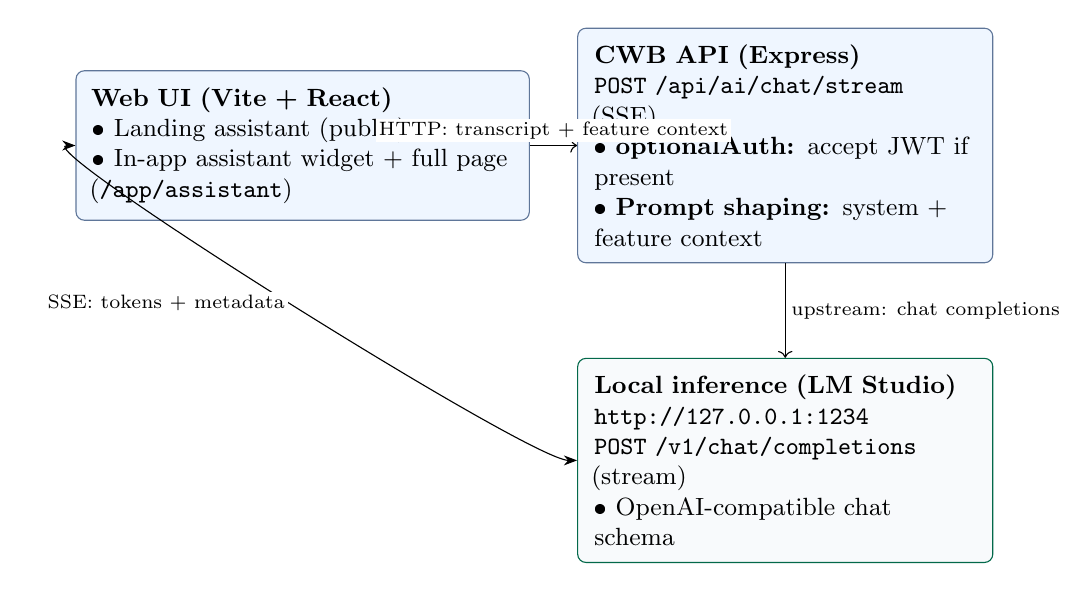
\begin{tikzpicture}[
  font=\small,
  node distance=8mm and 10mm,
  box/.style={draw=PrimaryBlue!70, rounded corners=3pt, align=left, inner sep=6pt, fill=LightBlue},
  server/.style={draw=GreenAccent!70!black, rounded corners=3pt, align=left, inner sep=6pt, fill=RowShade},
  smalllabel/.style={font=\scriptsize, inner sep=1pt, fill=white, draw=none},
  -{Stealth[length=2.2mm]}
]

\node[box, text width=0.44\linewidth] (ui) {%
  \textbf{Web UI (Vite + React)}\\
  \textbullet\ Landing assistant (public)\\
  \textbullet\ In-app assistant widget + full page (\texttt{/app/assistant})
};

\node[box, text width=0.40\linewidth, right=6mm of ui] (api) {%
  \textbf{CWB API (Express)}\\
  \texttt{POST /api/ai/chat/stream} (SSE)\\
  \textbullet\ \textbf{optionalAuth:} accept JWT if present\\
  \textbullet\ \textbf{Prompt shaping:} system + feature context
};

\node[server, text width=0.40\linewidth, below=12mm of api, anchor=north] (lm) {%
  \textbf{Local inference (LM Studio)}\\
  \texttt{http://127.0.0.1:1234}\\
  \texttt{POST /v1/chat/completions} (stream)\\
  \textbullet\ OpenAI-compatible chat schema
};

\draw[->] (ui.east) -- node[smalllabel, pos=0.5, sloped, above=1pt] {HTTP: transcript + feature context} (api.west);
\draw[->] (api.south) -- node[smalllabel, pos=0.5, right=1pt] {upstream: chat completions} (lm.north);
\draw[->, Stealth-Stealth] (lm.west) .. controls +(-0.6,0) and +(-0.6,0) .. node[smalllabel, pos=0.5, left=1pt] {SSE: tokens + metadata} (ui.west);

\end{tikzpicture}
\caption{Local LLM assistant data flow: browser UI streams from the CWB API, which proxies to a local OpenAI-compatible model server. The path is the same in principle for both landing and in-app UIs, with optional user context when authenticated.}
\label{fig:local-llm-tikz}
\end{figure}

\paragraph{Implementation analysis (brief).}
The integration is successful for the project prototype because it reuses a stable transport shape (chat-completions with streaming) and isolates the model vendor behind a single API route, allowing the user interface to remain a thin client. The main practical engineering challenges in local development were: (1) \textbf{process/port hygiene} to keep the API bound to a predictable port, (2) \textbf{CORS and same-origin} considerations when the UI and API run on different localhost ports, mitigated with a Vite dev proxy to \texttt{/api} and with permissive dev CORS policy on the API, and (3) \textbf{RPC provider selection} for wallet reads in the browser, where some public endpoints may fail browser CORS; pinning explicit public RPC endpoints avoids noisy failures unrelated to the chat feature.

\paragraph{Relationship to the earlier rule-based assistant (legacy).}
The repository also retains early keyword-routed \texttt{/api/chatbot} handlers used for initial prototyping; the LLM path is additive. This separation prevents regressions in deterministic demo endpoints while the conversational assistant evolves.

\begin{table}[H]
\centering
\TableImageMaxFit{table A.1.png}
\TableScreenshotEnd
\end{table}

\vspace{2pt}
\noindent\textit{\small This appendix table summarizes assistant integration components and configuration aspects used in the prototype (UI, API proxying, and local model server). The purpose is to make the implementation reproducible and to clarify which parts are prototype conveniences versus production requirements.}

\chapter{Smart Contract Capabilities}

The complete banking architecture is designed around nine modular contracts. The current prototype implements the core three-contract lending foundation, with the remaining six modules planned for the final thesis phase.

\textbf{Implemented contracts:}
\begin{itemize}[noitemsep]
\item \textbf{World Bank Reserve Contract:} Reserve custody, deposit handling, national bank registration, capital allocation to national banks, system pause and unpause, emergency withdrawal, and system statistics.
\item \textbf{National Bank Contract:} Local bank registration, borrowing from the World Bank reserve, capital allocation to local banks, and network status queries.
\item \textbf{Local Bank Contract:} Borrower registration, loan application processing, approval and rejection workflows, installment generation and payment processing, approver management, and user account management.
\end{itemize}

\textbf{Planned contracts (Final Thesis Phase):}
\begin{itemize}[noitemsep]
\item \textbf{SavingsVault Contract:} Standard savings account management, variable yield accrual, withdrawal processing, and deposit-to-lending pool integration.
\item \textbf{FixedDeposit Contract:} Term deposit creation, lock period enforcement, agreed APY accrual, early withdrawal penalty calculation, and maturity release.
\item \textbf{GroupLendingPool Contract:} Group formation, multi-signature consent recording, shared collateral management, per-member disbursement, mutual liability enforcement, and group credit history recording.
\item \textbf{FXModule Contract:} Oracle-priced currency conversion, spread calculation, dual-currency lending denomination support, and conversion audit trail.
\item \textbf{InsuranceFund Contract:} Premium collection, claims processing, default coverage disbursement, and fund reserve management.
\item \textbf{CurrentAccount Contract:} Transactional account management, atomic peer transfers, recurring payment scheduling, and payroll deposit handling.
\end{itemize}


%% %%%%%%%%%%%%%%%%%%%%%%%%%%%%%%%%%%%%%%%%%%%%%%%%%%%%%%%%%%%%
%% REFERENCES
%% %%%%%%%%%%%%%%%%%%%%%%%%%%%%%%%%%%%%%%%%%%%%%%%%%%%%%%%%%%%%
\chapter*{References}
\addcontentsline{toc}{chapter}{References}

{\small
\begin{enumerate}[label={[\arabic*]}]
\item S.~M. Werner, D.~Perez, L.~Gudgeon, A.~Klages-Mundt, D.~Harz, and W.~J. Knottenbelt, ``SoK: Decentralized Finance (DeFi),'' \textit{arXiv preprint arXiv:2101.08778}, 2022. [Online]. Available: \url{https://arxiv.org/abs/2101.08778}

\item S.~Bastankhah, M.~Hashemi, and W.~Shi, ``An Adaptive Data-Driven DeFi Borrow-Lending Protocol,'' \textit{Proc. IEEE Int. Conf. Blockchain}, 2023.

\item G.~Palaiokrassas, A.~Skoufis, and L.~Tassiulas, ``Leveraging Machine Learning for Multichain DeFi Fraud Detection,'' \textit{Proc. IEEE Int. Conf. Blockchain and Cryptocurrency (ICBC)}, 2023.

\item D.~Adom, E.~O. Acheampong, and M.~Boateng, ``LIME and SHAP: A Comparison of Model-Agnostic Approaches to Explainability in Loan Approval Systems,'' \textit{International Journal of Advanced Computer Science and Applications}, vol.~13, no.~11, 2022.

\item B.~W. Tan, ``Central Bank Digital Currency and Financial Inclusion,'' \textit{IMF Working Paper WP/23/69}, 2023. [Online]. Available: \url{https://www.imf.org/en/Publications/WP}

\item F.~T. Liu, K.~M. Ting, and Z.-H. Zhou, ``Isolation Forest,'' in \textit{Proc. IEEE Int. Conf. Data Mining (ICDM)}, pp.~413--422, 2008. DOI: \url{https://doi.org/10.1109/ICDM.2008.17}

\item N.~Atzei, M.~Bartoletti, and T.~Cimoli, ``A Survey of Attacks on Ethereum Smart Contracts (SoK),'' in \textit{Proc. Int. Conf. Principles of Security and Trust (POST)}, pp.~164--186, 2017. DOI: \url{https://doi.org/10.1007/978-3-662-54455-6_8}

\item S.~M. Lundberg and S.-I. Lee, ``A Unified Approach to Interpreting Model Predictions,'' in \textit{Advances in Neural Information Processing Systems (NeurIPS)}, pp.~4765--4774, 2017. [Online]. Available: \url{https://proceedings.neurips.cc/paper/2017/hash/8a20a8621978632d76c43dfd28b67767-Abstract.html}

\item P.~Bracke, A.~Datta, C.~Jung, and S.~Sen, ``Machine Learning Explainability in Finance: An Application to Default Risk Analysis,'' \textit{Bank of England Staff Working Paper No.~816}, 2019. [Online]. Available: \url{https://www.bankofengland.co.uk/working-paper/2019/machine-learning-explainability-in-finance}

\item R.~Beck, C.~M\"{u}ller-Bloch, and J.~L. King, ``Governance in the Blockchain Economy: A Framework and Research Agenda,'' \textit{Journal of the Association for Information Systems}, vol.~19, no.~10, pp.~1020--1034, 2018. DOI: \url{https://doi.org/10.17705/1jais.00518}

\item D.~Mhlanga, ``Blockchain Technology for Financial Inclusion and Sustainable Development,'' in \textit{Digital Financial Inclusion}, Springer, 2022.

\item OpenZeppelin, ``OpenZeppelin Contracts,'' 2024. [Online]. Available: \url{https://openzeppelin.com/contracts}

\item DefiLlama, ``Lending Protocols --- DeFi TVL and Protocol Rankings,'' 2024--2025. [Online]. Available: \url{https://defillama.com/protocols/lending}

\item World Bank, ``The Global Findex Database 2021: Financial Inclusion, Digital Payments, and Resilience,'' 2021. [Online]. Available: \url{https://www.worldbank.org/en/publication/globalfindex}

\item Aave, ``Aave Protocol Documentation,'' 2024. [Online]. Available: \url{https://docs.aave.com/}

\item Compound, ``Compound Protocol Documentation,'' 2024. [Online]. Available: \url{https://docs.compound.finance/}

\item BCOLBD 2025, ``Blockchain Olympiad Bangladesh: Guideline and Evaluation Scheme,'' 2025. [Online]. Available: \url{https://bcolbd.org/uploads/guideline/BLOCKCHAIN\%20OLYMPIAD\%20BANGLADESH\%20Blockchain\%20Guideline.pdf}

\item Galaxy Digital, ``The State of Crypto Lending and Borrowing,'' Galaxy Research, 2024. [Online]. Available: \url{https://www.galaxy.com/insights/research/the-state-of-crypto-lending}

\item World Bank, ``World Development Report 2022: Finance for an Equitable Recovery,'' 2022. [Online]. Available: \url{https://www.worldbank.org/en/publication/wdr2022}

\item International Finance Corporation (IFC), ``MSME Finance Gap 2019,'' 2019. [Online]. Available: \url{https://www.ifc.org/en/insights-reports/2019/msme-finance-gap}

\item Bank for International Settlements, ``DeFi Lending: Intermediation Without Information?,'' BIS Working Paper No.~1183, 2024. [Online]. Available: \url{https://www.bis.org/publ/work1183.pdf}

\item Deloitte, ``Global Banking Outlook 2024,'' 2024.

\item Michigan State University Libraries, ``Literature Table and Synthesis --- Nursing Literature Reviews,'' LibGuides, 2025. [Online]. Available: \url{https://libguides.lib.msu.edu/nursinglitreview/table}

\item Committee on Payments and Market Infrastructures and Bank for International Settlements, ``Correspondent Banking --- Technical Report,'' CPMI Papers No.~147, 2016. [Online]. Available: \url{https://www.bis.org/cpmi/publ/d147.pdf}

\item Ripple, ``RLUSD Use Case Analysis,'' XRP Academy, 2026. [Online]. Available: \url{https://xrpacademy.com/blog/rlusd-use-case-analysis-calendar-570}

\item World Bank, ``Remittance Prices Worldwide: Making Markets More Transparent,'' Migration and Development Brief~40, 2024. [Online]. Available: \url{https://remittanceprices.worldbank.org/}

\item DefiLlama, ``Aave V3 TVL, Fees, Revenue \& Income Statement,'' March 2026. [Online]. Available: \url{https://defillama.com/protocol/aave-v3}

\item World Inequality Lab, ``Exorbitant Privilege,'' \textit{World Inequality Report 2026}, 2026. [Online]. Available: \url{https://wir2026.wid.world/insight/exorbitant-privilege/}

\item DefiLlama, ``Compound V3 TVL, Fees, Revenue \& Income Statement,'' March 2026. [Online]. Available: \url{https://defillama.com/protocol/compound-v3}

\item Fensory, ``Sky Protocol Projects \$611M Revenue in 2026 as USDS Supply Targets \$20.6 Billion,'' February 2026. [Online]. Available: \url{https://www.fensory.com/intelligence/rwa/sky-protocol-tokenization-regatta-solana-february-2026}

\item Fensory, ``Maple Finance --- Institutional DeFi Lending Protocol,'' 2026. [Online]. Available: \url{https://www.fensory.com/insights/protocols/maple-finance}

\item Fensory, ``DeFi Credit Platforms Hit \$2.4B Milestone,'' March 2026. [Online]. Available: \url{https://www.fensory.com/intelligence/rwa/defi-private-credit-platforms-2-4-billion-loans-ethereum}

\item Financial Stability Board, ``Enhancing Cross-border Payments: Stage 3 Roadmap,'' 2020. [Online]. Available: \url{https://www.fsb.org/2020/10/enhancing-cross-border-payments-stage-3-roadmap/}

\item A.~Beyer, B.~Gasperini, and P.~Theodoridis, ``Monetary Policy and Inequality: Distributional Effects of Asset Purchase Programs,'' \textit{Journal of International Money and Finance}, vol.~157, 2025.

\item Federal Reserve Board, ``Monetary Policy and the Distribution of Income: Evidence from U.S. Metropolitan Areas,'' FEDS Notes, March 2025. [Online]. Available: \url{https://www.federalreserve.gov/econres/notes/feds-notes/monetary-policy-and-the-distribution-of-income-evidence-from-us-metropolitan-areas-20250331.html}

\item R.~Cantillon, \textit{Essai sur la Nature du Commerce en G\'en\'eral} (\textit{Essay on the Nature of Commerce in General}), 1755 (posthumous).

\item GlobeNewswire, ``R3's Corda Leads Tokenized RWA Market with Over \$10 Billion in On-chain Assets,'' February 2025. [Online]. Available: \url{https://www.globenewswire.com/news-release/2025/02/13/3025637/}

\item Centrifuge, ``Real-World Asset Tokenization: Key Trends from 2025,'' 2025. [Online]. Available: \url{https://centrifuge.io/blog/real-world-asset-tokenization-trends-2025}

\item World Bank, ``World Bank Group Tracks Project Funds with New Blockchain Tool,'' Press Release, September 2025. [Online]. Available: \url{https://www.worldbank.org/en/news/press-release/2025/09/26/world-bank-group-tracks-project-funds-with-new-blockchain-tool}

\item JPMorgan, ``Kinexys Digital Payments: Real-Time Multicurrency Payments,'' 2025. [Online]. Available: \url{https://www.jpmorgan.com/onyx/coin-system.htm}

\item World Economic Forum, ``Why Decentralized Finance Is a Leapfrog Technology for the 1.1 Billion People Who Are Unbanked,'' September 2022. [Online]. Available: \url{https://weforum.org/stories/2022/09/decentralized-finance-a-leapfrog-technology-for-the-unbanked}

\item Opera Newsroom, ``160M CELO Allocation Proposal to Grow Opera from Distribution Partner into Key Network Stakeholder,'' March 2026. [Online]. Available: \url{https://press.opera.com/2026/03/19/opera-celo-partnership-2026/}

\item Morpho, ``Network Data,'' March 2026. [Online]. Available: \url{https://data.morpho.org/}

\item Stellar, ``End of Year 2025 Report --- Execution at Scale,'' 2025. [Online]. Available: \url{https://www.stellar.org/blog/foundation-news/2025-year-in-review}

\item Human Rights Foundation, ``Tracking CBDCs Before They Track You,'' 2025. [Online]. Available: \url{https://hrf.org/latest/tracking-cbdcs-before-they-track-you}

\item Y.~Li, X.~Zhang, and H.~Wang, ``Design and Implementation of a Multi-Chain Lending Model in Blockchain,'' in \textit{Proc. IEEE Int. Conf. Blockchain}, 2024. DOI: \url{https://doi.org/10.1109/Blockchain62396.2024.10729983}

\item R.~Xu, S.~Chen, and L.~Yang, ``An Evaluation System for DeFi Lending Protocols,'' in \textit{Proc. IEEE Int. Conf. Blockchain and Cryptocurrency (ICBC)}, pp.~1--6, 2023. DOI: \url{https://doi.org/10.1109/ICBC56567.2023.10240601}

\item A.~Sharma, R.~K.~Singh, and S.~Gupta, ``Blockchain Empowered Framework for Peer to Peer Lending,'' in \textit{Proc. IEEE Int. Conf. Blockchain Computing and Applications (BCCA)}, pp.~142--147, 2021. DOI: \url{https://doi.org/10.1109/BCCA53669.2021.9596552}

\item M.~T.~Hassan, F.~Ahmad, and A.~Mehmood, ``Blockchain and Machine Learning for Fraud Detection: A Privacy-Preserving and Adaptive Incentive Based Approach,'' \textit{IEEE Access}, vol.~10, pp.~87115--87131, 2022. DOI: \url{https://doi.org/10.1109/ACCESS.2022.3199498}

\item Y.~Wang, J.~Liu, and Z.~Chen, ``ContractWard: Automated Vulnerability Detection Models for Ethereum Smart Contracts,'' \textit{IEEE Trans. Network Science and Engineering}, vol.~8, no.~2, pp.~1133--1144, 2020. DOI: \url{https://doi.org/10.1109/TNSE.2020.2968505}

\item C.-F.~Liao, T.-H.~Tsai, and C.-J.~Chen, ``SoliAudit: Smart Contract Vulnerability Assessment Based on Machine Learning and Fuzz Testing,'' in \textit{Proc. IEEE Int. Conf. Internet of Things (iThings)}, pp.~458--465, 2019. DOI: \url{https://doi.org/10.1109/iThings/GreenCom/CPSCom/SmartData.2019.00098}

\item S.~So, M.~Lee, J.~Park, H.~Lee, and H.~Oh, ``VERISMART: A Highly Precise Safety Verifier for Ethereum Smart Contracts,'' in \textit{Proc. IEEE Symp. Security and Privacy (S\&P)}, pp.~1678--1694, 2020. DOI: \url{https://doi.org/10.1109/SP40000.2020.00032}

\item S.~Islam, R.~Khan, and M.~A.~Rahman, ``Central Bank Digital Currency (CBDC): Design Requirements and Challenges,'' in \textit{Proc. IEEE Int. Conf. Computing, Communication, and Intelligent Systems (ICCCIS)}, 2024. DOI: \url{https://doi.org/10.1109/ICCCIS62002.2024.10634472}

\item M.~S.~Alam, S.~M.~Hossain, and A.~K.~Das, ``Towards Using Blockchain Technology for Microcredit Industry in Bangladesh,'' in \textit{Proc. IEEE Region 10 Symp. (TENSYMP)}, pp.~1--6, 2021. DOI: \url{https://doi.org/10.1109/TENSYMP52854.2021.9392730}

\item P.~Tolmach, Y.~Li, and S.~Lin, ``Optimal Gas Fee Minimization in DeFi: Enhancing Efficiency and Security on the Ethereum Blockchain,'' \textit{IEEE Trans. Dependable and Secure Computing}, 2024. DOI: \url{https://doi.org/10.1109/TDSC.2024.3495637}

\item S.~Gupta, A.~Kumar, and R.~Sharma, ``SHAP-based Interpretable Models for Credit Default Assessment Using Machine Learning,'' in \textit{Proc. IEEE Int. Conf. Artificial Intelligence and Data Science}, 2024. DOI: \url{https://doi.org/10.1109/ICAIDS60875.2024.10840375}

\item S.~Nakamoto, ``Bitcoin: A Peer-to-Peer Electronic Cash System,'' 2008. [Online]. Available: \url{https://bitcoin.org/bitcoin.pdf}

\item G.~Wood, ``Ethereum: A Secure Decentralised Generalised Transaction Ledger'' (Yellow Paper), Ethereum Foundation, 2014 (revised 2023). [Online]. Available: \url{https://ethereum.github.io/yellowpaper/paper.pdf}

\item Aave, ``Aave Protocol V3 Technical Paper,'' 2022. [Online]. Available: \url{https://github.com/aave/aave-v3-core/blob/master/techpaper/Aave_V3_Technical_Paper.pdf}

\item T.~Dao, T.~Trinh, and V.~Pham, ``Optimizing Credit Scoring Models for Decentralized Financial Applications,'' in \textit{Information and Communication Technology}, Springer, 2025. DOI: \url{https://doi.org/10.1007/978-981-96-4282-3_36}

\item G.-L.~G\"{u}c\"{u}k, S.~Leible, and J.~Edinger, ``Blockchain-Based Microlending for Financial Inclusivity: A Literature Review of Its Privacy and Trust,'' Springer, 2024. DOI: \url{https://doi.org/10.1007/978-3-032-12801-0_22}
\end{enumerate}
}

\end{document}